% -*- coding: utf-8 -*-

\begin{chapter}{Уравнения движения вязкой жидкости}\label{chap:8}
% \chapter{Equations of Motion With Viscosity}

Силы трения, действующие в океане и атмосфере, практически во всем их объеме
оказываются настолько малыми по сравнению с прочими силами, что мы можем 
не принимать их во внимание. В то же время, на границе двух сред влияние трения, 
проявляющееся в форме вязкости, становится существенным.
Этот тонкий вязкий слой называется 
\emph{пограничным слоем}\index{пограничный слой|textbf}. Скорость потока 
уменьшается внутри пограничного слоя от величин, характерных для потока в
толще жидкости, до нуля на границе с твёрдым телом. Пограничный слой 
на границе раздела двух несмешивающихся жидкостей представляет собой 
тонкий слой, скорость движения в котором быстро изменяется таким образом, 
чтобы скорость по одну сторону границы была согласована со скоростью на 
противоположной её стороне. Примером пограничного слоя может служить
расположенный в нижней части атмосферы планетарный пограничный слой, 
рассмотренный нами в гл.~\ref{chap:4}.
Внутри планетарного пограничного слоя скорости снижаются со многих
метров в секунду в свободной атмосфере до десятков сантиметров в
секунду над поверхностью моря. По другую сторону этой поверхности находится
еще один пограничный слой, слой Экмана\index{Экмана слой}, который 
связывает поток на поверхности океана с более глубокими слоями,
о чем будет подробнее сказано в гл.~\ref{chap:9}.
%
% Throughout most of the interior of the ocean and atmosphere friction
% is relatively small, and we can safely assume that the flow is
% frictionless. At the boundaries, friction, in the form of viscosity,
% becomes important. This thin, viscous layer is called a
% \textit{boundary layer}\index{boundary layer|textbf}. Within the
% layer, the velocity slows from values typical of the interior to zero
% at a solid boundary. If the boundary is not solid, then the boundary
% layer is a thin layer of rapidly changing velocity whereby velocity on
% one side of the boundary changes to match the velocity on the other
% side of the boundary. For example, there is a boundary layer at the
% bottom of the atmosphere, the planetary boundary layer I described in
% Chapter 3. In the planetary boundary layer, velocity goes from many
% meters per second in the free atmosphere to tens of centimeters per
% second at the sea surface. Below the sea surface, another boundary
% layer, the \index{Ekman layer}Ekman layer described in Chapter 9,
% matches the flow at the sea surface to the deeper flow.

В этой главе мы обсудим влияние трения на потоки жидкости, а также
устойчивость потоков к небольшим изменениям скорости или плотности.
%
% In this chapter I consider the role of friction in fluid flows, and
% the stability of the flows to small changes in velocity or density.

\begin{section}{Влияние вязкости}
% \section{The Influence of Viscosity}
Вязкость\index{вязкость} жидкости характеризует ее сопротивление сдвиговой
деформации. В предыдущей главе мы записали компоненту уравнения движения 
жидкости по оси~$x$ в форме~(\ref{eq:7.12a}):
\begin{equation}\label{eq:8.1}
\frac{\partial{u}}{\partial{t}}+u\,\frac{\partial{u}}{\partial{x}}
 +v\,\frac{\partial{u}}{\partial{y}}+w\,\frac{\partial{u}}{\partial{z}}
=-\,\frac{1}{\rho}\frac{\partial{p}}{\partial{x}} + 2\,\Omega\,v\,\sin\vartheta + F_x,
\end{equation}
где через $F_x$ обозначена массовая сила трения. Рассмотрим, как
будет выглядеть это слагаемое, если предположить, что данная сила возникает 
под влиянием вязкости.
%
% \index{viscosity}Viscosity is the tendency of a fluid to resist
% shear. In the last chapter I wrote the $x$--component of the momentum
% equation for a fluid in the form (7:12a):
% \begin{equation}
% \frac{\partial{u}}{\partial{t}}+u\,\frac{\partial{u}}{\partial{x}}+v\,
% \frac{\partial{u}}{\partial{y}}+w\,\frac{\partial{u}}{\partial{z}}=-\,
% \frac{1}{\rho}\frac{\partial{p}}{\partial{x}} + 2\,\Omega\,v\,\sin\vartheta + F_x
% \end{equation}
% where $F_x$ was a frictional force per unit mass. Now we can consider
% the form of this term if it is due to viscosity.

Молекулы жидкости, находящиеся около границы твёрдого тела, могут 
время от времени сталкиваться с ним и передавать ему импульс 
(рис.~\ref{fig:viscositysketch}). Далее эти молекулы могут также столкнуться 
с другими молекулами жидкости, не имеющими непосредственного контакта 
с границей, что ведет, в свою очередь, к передаче изменения импульса 
внутрь потока. Подобный перенос импульса принято называть
\emph{молекулярной вязкостью}\index{молекулярная вязкость|textbf}%
\index{вязкость!молекулярная|textbf}. Однако, величина пробега молекул между
столкновениями составляет около микрометра, и процесс этот
неэффективен для передачи импульса даже на расстояние порядка нескольких
сантиметров. Таким образом, молекулярная вязкость важна только только 
при удалении от границы не более чем на несколько миллиметров.
%
% Molecules in a fluid close to a solid boundary sometime strike the
% boundary and transfer momentum to it (figure 8.1). Molecules further
% from the boundary collide with molecules that have struck the
% boundary, further transferring the change in momentum into the
% interior of the fluid. This transfer of momentum is 
% \textit{molecular viscosity}\index{molecular
% viscosity|textbf}\index{viscosity!molecular|textbf}. Molecules,
% however, travel only micrometers between collisions, and the process
% is very inefficient for transferring momentum even a few
% centimeters. Molecular viscosity is important only within a few
% millimeters of a boundary.

Молекулярная вязкость~$\rho \nu$ определяется как отношение напряжения~$T$,
направленного по касательной к границе потока, и сдвига скорости
на границе. Следовательно, напряжение имеет вид:
\begin{equation}\label{eq:8.2}
T_{xz} =  \rho \nu \,\frac{\partial{u}}{\partial{z}}
\end{equation}
при условии, что поток движется в плоскости~$(x, z)$ на расстоянии нескольких
миллиметров от поверхности, а~$\nu$~--- кинематическая молекулярная вязкость. 
Типичные значения~$\nu$ для воды при~$\degCent{20}$ составляют~$10^{-6}\sqmps$.
%
% Molecular viscosity $\rho \nu$ is the ratio of the stress $T$
% tangential to the boundary of a fluid and the velocity shear at the
% boundary. So the stress has the form:
% \begin{equation}
% T_{xz} =  \rho \nu \,\frac{\partial{u}}{\partial{z}}
% \end{equation}
% for flow in the $(x, z)$ plane within a few millimetres of the
% surface, where $\nu$ is the kinematic molecular viscosity. Typically
% $\nu = 10^{-6}$ m$^2$/s for water at 20\degrees{C}.

Обобщение~(\ref{eq:8.2}) на три измерения даёт нам тензор турбулентных 
напряжений, включающий девять компонент напряжения в точке жидкости, 
в том числе давление (нормальное напряжение) и сдвиговые напряжения. Вывод
этого тензора выходит за рамки задач, стоящих перед данным пособием; 
подробности, при необходимости, могут быть найдены в 
работах Lamb (1945: \S 328) 
%% у Ламба в этом параграфе нет ни слова про "тензор напряжения"
или Kundu (1990: p. 93). 
В случае несжимаемой жидкости массовая сила трения в~(\ref{eq:8.1}) примет
вид:
\begin{equation}
F_x= \frac{\partial }{\partial x} \left[ \nu \frac{\partial u}{\partial x} \right]
   + \frac{\partial }{\partial y} \left[ \nu \frac{\partial u}{\partial y} \right]
   + \frac{\partial }{\partial z} \left[ \nu \frac{\partial u}{\partial z} \right]
= \frac{1}{\rho} \left[ \frac{\partial T_{xx}}{\partial x} +
                        \frac{\partial T_{xy}}{\partial y} +
                        \frac{\partial T_{xz}}{\partial z} \right].
\end{equation}
%
% Generalizing (8.2) to three dimensions leads to a stress tensor giving
% the nine components of stress at a point in the fluid, including
% pressure, which is a normal stress, and shear stresses. A derivation
% of the stress tensor is beyond the scope of this book, but you can
% find the details in Lamb (1945: \S 328) or Kundu (1990: p. 93). For an
% incompressible fluid, the frictional force per unit mass in (8.1)
% takes the form:
% \begin{equation}
% F_x= \frac{\partial }{\partial x} \left[ \nu \frac{\partial u}{\partial x} \right]
%    + \frac{\partial }{\partial y} \left[ \nu \frac{\partial u}{\partial y} \right]
%    + \frac{\partial }{\partial z} \left[ \nu \frac{\partial u}{\partial z} \right]
% = \frac{1}{\rho} \left[ \frac{\partial T_{xx}}{\partial x} +
%                         \frac{\partial T_{xy}}{\partial y} +
%                         \frac{\partial T_{xz}}{\partial z} \right]
% \end{equation}

%% В оригинале отсутствует:
%%Эта форма члена трения в уравнении движения была впервые опубликована
%%Навье (1785--1836) в 1827 году.

\begin{figure}[t!]
\makebox [120mm][c]{\includegraphics{pics/viscositysketch}}
\caption{Молекулы, сталкиваясь со стенкой и друг с другом, передают
импульс потока стенке, замедляя скорость движения
жидкости.}
\label{fig:viscositysketch}
\end{figure}
%
% \begin{figure}[t!]
% \makebox[120mm] [c]{\includegraphics{viscositysketch}}
% \centering
% \footnotesize
% Figure 8.1 Molecules \rule{0mm}{4ex}colliding with the wall and with
% each other transfer\\momentum from the fluid to the wall, slowing the
% fluid velocity.
%
% \label{fig:viscositysketch}
% \vspace{-3ex}
% \end{figure}

\begin{figure}[t!]
\makebox[120mm] [c]{\includegraphics{pics/reynoldsexp}}
\caption{Аппарат Рейнольдса для исследования турбулентности, возникающей
в потоке жидкости, а также фотографии потока, 
близкого к ламинарному (вверху) и турбулентного (внизу), в прозрачной трубке, 
похожей на ту, которую использовал Рейнольдс (From Binder 1953).}
\label{fig:reynoldsexp}
\end{figure}
%
% \begin{figure}[t!]
% \makebox[120mm] [c]{\includegraphics{reynoldsexp}}
% \footnotesize
% Figure 8.2 Reynolds \rule{0mm}{4ex}apparatus for investigating the
% transition to turbulence\index{turbulence!transition to} in pipe flow,
% with photographs of near-laminar flow (left) and turbulent flow
% (right) in a clear pipe much like the one used by Reynolds. After
% Binder (1949: 88-89).
% \label{fig:reynoldsexp}
% \vspace{-4ex}
% \end{figure}
\end{section}

\begin{section}{Турбулентность}\label{sec:turbulence}
% \section{Turbulence}
\index{вязкость!турбулентная}Если молекулярная вязкость важна только 
на расстоянии в несколько миллиметров и, с точки зрения наблюдателя 
крупнее зоопланктона, не играет роли в большинстве океанических потоков,
то каким же образом влияние границы передаётся внутрь потока? 
Ответ: через турбулентность.
%
% \index{viscosity!turbulent}If molecular viscosity is important only
% over distances of a few millimeters, and if it is not important for
% most oceanic flows, unless of course you are a zooplankter trying to
% swim in the ocean, how then is the influence of a boundary transferred
% into the interior of the flow? The answer is: through turbulence.

Турбулентность является следствием наличия в уравнении количества движения
нелинейных членов ($u\,\partial{u}/\partial{x}$, и др.). Их вклад
характеризуется безразмерным числом Рейнольдса, 
которое представляет собой отношение нелинейного и диссипативного членов
в уравнении Навье-Стокса%
\remark{\href{http://ru.wikipedia.org/wiki/\%D0\%A0\%D0\%B5\%D0\%B9\%D0\%BD\%D0\%BE\%D0\%BB\%D1\%8C\%D0\%B4\%D1\%81\%D0\%B0_\%D1\%87\%D0\%B8\%D1\%81\%D0\%BB\%D0\%BE}%
{<<Число Рейнольдса>>, Википедия}}:
\begin{equation}
\Reyn = \frac{\text{Нелинейный член}}{\text{Диссипативный член}} 
      = \cfrac{\left(u\,\cfrac{\partial{u}}{\partial{x}}\right) }%
              {\left(\nu\,\cfrac{\partial^2{u}}{\partial{x^2}}\right)} 
      \approx \cfrac{U\,\cfrac{U}{L\vphantom{y}}}{\nu\,\cfrac{U}{L^2}}
      = \frac{UL}{\nu},
\end{equation}
где $U$~--- характерная скорость потока, а $L$~--- его характерный размер.
Выбор $U$ и~$L$ произволен, но эти величины должны быть типичными для данного 
потока. Например, $L$ может быть или средним поперечным, или продольным
размером потока. Для открытого океана характерны $U=0.1\mps$ 
и~$L=1~\text{мегаметр}$, откуда~$\Reyn=10^{11}$. Так как влияние нелинейных 
компонент становится важным при $\Reyn > 10, \ldots, 1000$, то в нашем случае
они, очевидно, важны, и океан следует полагать турбулентным.
%
% Turbulence arises from the non-linear terms in the momentum equation
% $(u\,\partial{u}/\partial{x}$, \textit{etc}.). The importance of these
% terms is given by a non-dimensional number, the Reynolds Number $Re$,
% which is the ratio of the non-linear terms to the viscous terms:
% \begin{equation}
% Re = \frac{\text{Non-linear Terms}}{\text{Viscous
% Terms}} =
% \cfrac{\left( \displaystyle u\,\cfrac{\partial{u}}{\partial{x}}\right) }{\left( \displaystyle \nu\,\cfrac{\partial^2{u}}{\partial{x^2}}\right)
% } \approx \cfrac{\D U\,\cfrac{U}{L\vphantom{y}}}{\D \nu\,\cfrac{U}{L^2}}
% = \frac{UL}{\nu}
% \end{equation}
% where, $U$ is a typical velocity of the flow and $L$ is a typical length
% describing the flow. You are free to pick whatever $U,L$ might be typical of
% the flow. For example $L$ can be either a typical cross-stream distance, or an
% along-stream distance. Typical values in the open ocean are $U = 0.1$ m/s and
% $L = 1$ megameter, so $Re = 10^{11}$. Because non-linear terms are important if
% Re $>$ 10 -- 1000, they are certainly important in the ocean. The ocean is
% turbulent.

Число Рейнольдса названо в честь Осборна Рейнольдса (1842--1912),
проводившего в конце XIX~в.\ эксперименты, призванные помочь понять
турбулентность\index{турбулентность!измерение}. Один из них, получивший 
широкую известность (Reynolds 1883), состоял в том, в воду, 
текущую с разной скоростью через трубку, вводился краситель 
(рис.~\ref{fig:reynoldsexp}). Течение было спокойным (или \emph{ламинарным})
на малой скорости, а с её ростом становилось нерегулярным и турбулентным. 
Переход от одного состояния к другому происходил 
при~$\Reyn = VD/\nu \approx 2000$, где $V$~--- средняя
скорость в трубке, а $D$~--- её диаметр.
%
% The Reynolds number is named after Osborne Reynolds (1842--1912) who
% conducted experiments in the late 19th century to understand
% turbulence\index{turbulence!measurement of}.  In one famous experiment
% (Reynolds 1883), he injected dye into water flowing at various speeds
% through a tube (figure 8.2). If the speed was small, the flow was
% smooth. This is called \textit{laminar flow}. At higher speeds, the
% flow became irregular and turbulent. The transition occurred at Re $ =
% VD/\nu \approx 2000$, where $V$ is the average speed in the pipe, and
% $D$ is the diameter of the pipe.

Когда число Рейнольдса превышает некоторое критическое значение, 
течение становится всё более и более турбулентным. Отметим, что характер
потока является функцией числа Рейнольдса. Все течения с
одинаковой геометрией и одинаковым числом Рейнольдса обладают
одинаковой структурой потока. Таким образом, течение вокруг всех
круговых цилиндров, будь они $1\mm$ или~$1\m$ в диаметре, при условии равенства
числа Рейнольдса~$20$, будет напоминать приведенное в верхней части 
рис.~\ref{fig:turbsketch}. Также отметим, что пограничный слой очень 
близко прилегает к цилиндру и слишком тонок, чтобы быть показанным на рисунке.
%
% As Reynolds number increases above some critical value, the flow
% becomes more and more turbulent. Note that flow pattern is a function
% of Reynold's number. All flows with the same geometry and the same
% Reynolds number have the same flow pattern. Thus flow around all
% circular cylinders, whether 1 mm or 1 m in diameter, look the same as
% the flow at the top of figure 8.3 if the Reynolds number is
% 20. Furthermore, the boundary layer is confined to a very thin layer
% close to the cylinder, in a layer too thin to show in the figure.

\begin{figure}[t!]
\makebox[120mm][c]{\includegraphics{pics/turbsketch}}
\caption{Форма потока, обтекающего круговой цилиндр, как функция числа
Рейнольдса в диапазоне от единицы до миллиона (From Richardson 1961). 
A~--- зубочистка в потоке~$1\mmps$; B~--- палец в потоке~$2\cmps$; 
F~--- рука, высунутая из окна на скорости 60 миль/час. 
Линии тока течений с одинаковым числом Рейнольдса выглядят одинаково. 
Поток, обтекающий цилиндр диаметром~$10\cm$ со скоростью~$1\cmps$, выглядит 
так же, как поток со скоростью~$10\cmps$, обтекающий цилиндр 
диаметром~$1\cm$, поскольку в обоих случаях $\Reyn = 1000$.}
\label{fig:turbsketch}
\vspace{-2ex}
\end{figure}
%
% \begin{figure}[t!]
% \makebox[120mm][c]{\includegraphics{turbsketch}}
% \footnotesize
% Figure 8.3 Flow past a circular \rule{0mm}{3ex}cylinder as a function
% of Reynolds number between one and a million. From Richardson
% (1961). The appropriate flows are: A---a toothpick moving at 1 mm/s;
% B---finger moving at 2 cm/s; F---hand out a car window at 60 mph. All
% flow at the same Reynolds number has the same streamlines. Flow past a
% 10 cm diameter cylinder at 1 cm/s looks the same as 10 cm/s flow past
% a cylinder 1 cm in diameter because in both cases Re $= 1000$.
% \label{fig:turbsketch}
% \vspace{-2ex}
% \end{figure}

\begin{paragraph}{Турбулентное напряжение: напряжение Рейнольдса.}
% \paragraph{Turbulent Stresses: The Reynolds Stress}
\index{турбулентное!напряжение}\index{Рейнольдса напряжение}%
Прандтль, Карман и другие исследователи, изучавшие гидромеханику в начале
XX~ст.\, предполагали, что в турбулентном течении малые объёмы жидкости 
играют при передаче импульса внутрь течения такую же роль, какую 
молекулы~--- в ламинарном. Исследования в этом направлении привели 
к понятию турбулентных напряжений.
%
% \index{turbulent!stress}\index{Reynolds Stress}Prandtl, Karman and
% others who studied fluid mechanics in the early 20th century,
% hypothesized that parcels of fluid in a turbulent flow played the same
% role in transferring momentum within the flow that molecules played in
% laminar flow. The work led to the idea of turbulent stresses.

Чтобы увидеть, каким образом могут возникать подобные напряжения, рассмотрим
уравнение движения для потока, в котором выделены средняя~$(U, V, W)$ 
и турбулентная~$(u', v', w')$ компоненты:
\begin{equation}\label{eq:8.5}
 u=U+u' \,;\quad v = V+v' \,;\quad w=W+w' \, ;\quad p=P+p',
\end{equation}
где значение~$U$ вычислено осреднением по пространству и времени:
\begin{equation}
U = \langle u \rangle =\frac{1}{T}\int^T_0\,u(t)\,dt \quad \text{либо}\quad
U = \langle u \rangle =\frac{1}{X}\int^X_0\,u(x)\,dx
\end{equation}
%
% To see how these stresses might arise, consider the momentum equation
% for a flow with mean $(U, V, W)$ and turbulent $(u', v', w')$
% components:
% \begin{equation}
% u=U+u' \,;\quad v = V+v' \,;\quad w=W+w' \, ;\quad p=P+p'
% \end{equation}
% where the mean value $U$ is calculated from a time or space average:
% \begin{equation}
% U = \langle u \rangle =\frac{1}{T}\int^T_0\,u(t)\,dt \quad \text{or}\quad
% U = \langle u \rangle =\frac{1}{X}\int^X_0\,u(x)\,dx
% \end{equation}

Нелинейные члены уравнения количества движения могут быть записаны как
\begin{align}\label{eq:8.7}
\left< (U+u')\frac{\partial{(U+u')}}{\partial{x}} \right> 
  &= \left< U\,\frac{\partial{U}}{\partial{x}}\right> 
     + \left< U\,\frac {\partial{u'}}{\partial{x}}\right> 
     + \left< u' \,\frac {\partial{U}}{\partial{x}}\right> 
     + \left< u' \,\frac {\partial{u'}}{\partial{x}}\right> \notag \\
\left< (U+u')\frac{\partial{(U+u')}}{\partial{x}} \right> 
  &= \left< U\,\frac{\partial{U}}{\partial{x}}\right> 
    + \left<u' \,\frac{\partial{u'}}{\partial{x}}\right>.
\end{align}
Второе уравнение следует из первого, так как 
и $\langle U\,\partial{u'}/\partial{x}\rangle = 0$, 
и $\langle u'\,\partial{U}/\partial{x}\rangle = 0$, 
поскольку по определению $U$:
$\langle U \partial{u'}/\partial{x}\rangle 
 = U \partial{\langle u' \rangle }/\partial{x} = 0$.
%
% The non-linear terms in the momentum equation can be written:
% \begin{align}
% \left< (U+u')\frac{\partial{(U+u')}}{\partial{x}} \right> &= \left<
% U\,\frac{\D \partial{U}}{\partial{x}}\right> +
% \left< U\,\frac {\partial{u'}}{\partial{x}}\right> +
% \left< u' \,\frac {\partial{U}}{\partial{x}}\right> + \left< u' \,\frac
% {\partial{u'}}{\partial{x}}\right> \notag \\
% \left< (U+u')\frac{\partial{(U+u')}}{\partial{x}} \right> &= \left<
% U\,\frac{\D \partial{U}}{\partial{x}}\right> +
% \left<u' \,\frac{\partial{u'}}{\partial{x}}\right>
% \end{align}
% The second equation follows from the first since $\langle
% U\,\partial{u'}/\partial{x}\rangle = 0$ and $\langle
% u'\,\partial{U}/\partial{x}\rangle$ $= 0$, which follow from the
% definition of $U$: $\langle U \partial{u'}/\partial{x}\rangle = U
% \partial{\langle u' \rangle }/\partial{x}$ $ = 0$.

Применив~(\ref{eq:8.5}) к~(\ref{eq:7.19}), получим:
\begin{equation}\label{eq:8.8}
  \frac{\partial{U }}{\partial{x}} + \frac{\partial{V }}{\partial{y}}
 +\frac{\partial{W }}{\partial{z}} + \frac{\partial{u'}}{\partial{x}} 
 +\frac{\partial{v'}}{\partial{y}} + \frac{\partial{w'}}{\partial{z}} = 0.
\end{equation}
Вычитая среднее~(\ref{eq:8.8}) из~(\ref{eq:8.8}), разделим уравнение 
непрерывности на два:
\begin{subequations}
\begin{align}
\frac{\partial{U }}{\partial{x}} 
 + \frac{\partial{V }}{\partial{y}} 
 + \frac{\partial{W }}{\partial{z}} &=0 \\
\frac{\partial{u'}}{\partial{x}} 
 + \frac{\partial{v'}}{\partial{y}} 
 + \frac{\partial{w'}}{\partial{z}} &=0
\end{align}
\end{subequations}
%
% Using (8.5) in (7.19) gives:
% \begin{equation}
% \frac{\partial{U }}{\partial{x}} + \frac{\partial{V }}{\partial{y}}  +\frac{\partial{W }}{\partial{z}} + 
% \frac{\partial{u'}}{\partial{x}} + \frac{\partial{v'}}{\partial{y}}
% +\frac{\partial{w'}}{\partial{z}} =0
% \end{equation}
% Subtracting the mean of (8.8) from (8.8) splits the continuity
% equation into two equations:
% \begin{subequations}
% \begin{align}
% \frac{\partial{U }}{\partial{x}} + \frac{\partial{V }}{\partial{y}}  +\frac{\partial{W }}{\partial{z}} &= 0 \\
% \frac{\partial{u'}}{\partial{x}} + \frac{\partial{v'}}{\partial{y}} +\frac{\partial{w'}}{\partial{z}} &=0
% \end{align}
% \end{subequations}

Применив~(\ref{eq:8.5}) к~(\ref{eq:8.1}), осредним полученное уравнение
и упростим его при помощи~(\ref{eq:8.7}), после чего получим следующее
выражение для $x$-компоненты уравнения количества движения осредненного потока:
\begin{equation}\label{eq:8.10}
\begin{split}
\frac{DU}{Dt} & = -\frac{1}{\rho}\,\frac{\partial{P}}{\partial{x}}  + 2\Omega V\sin\varphi \\
  & + \frac{\partial }{\partial x} \left[ \nu \frac{\partial U}{\partial x} - \langle u'u'\rangle \right]
    + \frac{\partial }{\partial y} \left[ \nu \frac{\partial U}{\partial y} - \langle u'v'\rangle \right] +
      \frac{\partial }{\partial z} \left[ \nu \frac{\partial U}{\partial z} - \langle u'w'\rangle \right].
\end{split}
\end{equation}
Вывод данного соотношения не так прост, как может показаться на первый взгляд
(подробнее он рассмотрен в работе Hinze (1975: 22)). Исходя из сказанного выше,
дополнительная массовая сила будет составлять
\begin{equation}
F_x=-\frac{\partial}{\partial{x}}\langle u'u' \rangle
-\frac{\partial}{\partial{y}}\langle u'v' \rangle
-\frac{\partial}{\partial{z}}\langle u'w'\rangle.
\end{equation}
%
% Using (8.5) in (8.1) taking the mean value of the resulting equation,
% then simplifying using (8.7), the x-component of the momentum equation
% for the mean flow becomes:
% \begin{equation}
% \begin{split}
% \frac{DU}{Dt} & = -\frac{1}{\rho}\,\frac{\partial{P}}{\partial{x}}  + 2\Omega V\sin\varphi \\
%   & + \frac{\partial }{\partial x} \left[ \nu \frac{\partial U}{\partial x} - \langle u'u'\rangle \right]
%     + \frac{\partial }{\partial y} \left[ \nu \frac{\partial U}{\partial y} - \langle u'v'\rangle \right] +
%       \frac{\partial }{\partial z} \left[ \nu \frac{\partial U}{\partial z} - \langle u'w'\rangle \right]
% \end{split}
% \end{equation}
% The derivation is not as simple as it seems. See Hinze (1975: 22) for
% details. Thus the additional force per unit mass due to the
% turbulence\index{turbulent!stress} is:
% \begin{equation}
% F_x=-\frac{\partial}{\partial{x}}\langle u'u' \rangle
% -\frac{\partial}{\partial{y}}\langle u'v' \rangle
% -\frac{\partial}{\partial{z}}\langle u'w'\rangle
% \end{equation}

Члены $\rho{\langle u' u' \rangle}$, $\rho{\langle u' v'\rangle}$, и
$\rho{\langle u' w' \rangle}$ передают импульс~$\rho u' $, направленный
на восток, в направлениях $x$, $y$ и~$z$. Например, 
член $\rho{\langle u' w'\rangle}$ описывает направленный вниз перенос
направленного на восток импульса через горизонтальную плоскость. 
Так как эти члены характеризуют передачу импульса и были впервые выведены
Рейнольдсом, то они получили название 
\emph{напряжений Рейнольдса}\index{Рейнольдса напряжение|textbf}.
%
% The terms $\rho{\langle u' u' \rangle}$, $\rho{\langle u' v'
% \rangle}$, and $\rho{\langle u' w' \rangle}$ transfer eastward
% momentum ($\rho u' $) in the $x$, $y$, and $z$ directions. For
% example, the term $\rho{\langle u' w' \rangle}$ gives the downward
% transport \index{transport!momentum}of eastward momentum across a
% horizontal plane. Because they transfer momentum, and because they
% were first derived by Osborne Reynolds, they are called
% \textit{Reynolds Stresses}\index{Reynolds Stress|textbf}.
\end{paragraph}
\end{section}

\begin{section}{Расчёт напряжений Рейнольдса}
% \section{Calculation of Reynolds Stress:}
\index{Рейнольдса напряжение!вычисление}%
Напряжения Рейнольдса, такие как $\partial{\langle u'w'\rangle}/\partial{z}$,
называются виртуальными напряжениями (см.\ также Goldstein, 1965: \S{}69, \S{}80),
поскольку мы полагаем, что они играют роль, аналогичную диссипативным членам в 
уравнении движения. В дальнейшем нам потребуются значения либо функциональные
выражения напряжений Рейнольдса. Для их получения могут использоваться 
несколько различных подходов.
%
% \index{Reynolds Stress!calculation of}The Reynolds stresses such as
% $\partial{\langle u'w'\rangle}/\partial{z}$ are called virtual
% stresses (cf. Goldstein, 1965: \S 69 \& \S 81) because we assume that
% they play the same role as the viscous terms in the equation of
% motion. To proceed further, we need values or functional form for the
% Reynolds stress. Several approaches are used.

\begin{paragraph}{Экспериментальный подход.}
% \paragraph{From Experiments}
Напряжения Рейнольдса могут быть рассчитаны по непосредственным 
измерениям ($u', v', w'$), сделанным в лабораторных условиях либо в океане.
Этот метод достаточно точен, но трудно поддается обобщению на другие виды 
потоков. Следовательно, нам следует рассмотреть более общие подходы.
%
% We can calculate Reynolds stresses from direct measurements of ($u',
% v', w'$) made in the laboratory or ocean. This is accurate, but hard
% to generalize to other flows. So we seek more general approaches.
\end{paragraph}

\begin{paragraph}{Аналогия с молекулярной вязкостью.}
% \paragraph{By Analogy with Molecular Viscosity}
Обратимся еще раз к примеру, изображённому на рис.~\ref{fig:viscositysketch}, 
который демонстрирует пограничный слой над поверхностью, лежащей в 
плоскости $x$, $y$. В 1904~г.\ Прандтлем была опубликована революционная 
работа, в которой он высказал предположение, что turbulent viscous effects
играют заметную роль исключительно в тонком слое, близком к поверхности,
т.~е.\ в пограничном слое. Понятие пограничного слоя, введенное Прандтлем,
позволит нам с высокой точностью описать турбулентные потоки ветра над
морской поверхностью, а также потоки в придонном пограничном слое океана и
в перемешанном слое\index{перемешанный слой} на его поверхности.
(См.\ врезку <<Турбулентный пограничный слой над плоской поверхностью>>.)
%
% Let's return to the example in figure 8.1, which shows flow above a
% surface in the $x$, $y$ plane. Prandtl, in a revolutionary paper
% published in 1904, stated that turbulent viscous effects are only
% important in a very thin layer close to the surface, the boundary
% layer. Prandtl's invention of the boundary layer allows us to describe
% very accurately turbulent flow of wind above the sea surface, or flow
% at the bottom boundary layer in the ocean, or flow in the mixed
% layer\index{mixed layer} at the sea surface. See the box
% \textit{Turbulent Boundary Layer Over a Flat Plate}.

Чтобы рассчитать поток в пограничном слое, предположим, что течение 
над границей постоянно в направлении $x$, $y$, что
статистические свойства потока изменяются только по направлению $z$, и
что осредненное течение установившееся. Следовательно,
$\partial /\partial t = \partial /\partial x = \partial /\partial y = 0$
и~(\ref{eq:8.10}) может быть представлено в виде:
\begin{equation}
2 \Omega V \sin \varphi + \frac{\partial }{\partial z} 
 \left[\nu \frac{\partial U}{\partial z} - \langle u'w'\rangle \right] = 0.
\end{equation}
%
% To calculate flow in a boundary layer, we assume that flow is constant
% in the $x$, $y$ direction, that the statistical properties of the flow
% vary only in the $z$ direction, and that the mean flow is
% steady. Therefore $\partial /\partial t = \partial /\partial x =
% \partial /\partial y = 0$, and (8.10) can be written:
% \begin{equation}
% 2 \Omega V \sin \varphi + \frac{\partial }{\partial z} \left[\nu \frac{\partial
% U}{\partial z} - \langle u'w'\rangle \right] = 0
% \end{equation}

Далее по аналогии с~(\ref{eq:8.2}) предположим, что
\begin{equation}\label{eq:8.13}
- \rho \langle u'w'\rangle = T_{xz} = \rho A_z \frac{\partial U}{\partial z},
\end{equation}
где~$A_z$~--- это \emph{вихревая вязкость}
\index{вихревая вязкость|textbf}\index{вязкость!вихревая|textbf} 
или \emph{коэффициент вихревой диффузии}\index{вихревой диффузии коэффициент|textbf},
которая заменяет молекулярную вязкость~$\nu$ в уравнении~(\ref{eq:8.2}). Тогда
\begin{equation} 
\frac{\partial{T_{xz}}}{\partial{z}} 
 = \frac{\partial}{\partial{z}}\left(A_z\frac{\partial{U}}{\partial{z}}\right)
 \approx A_z \frac{\partial^2 U}{\partial z^2},
\end{equation}
предполагая $A_z$ или постоянной, или изменяющейся в направлении $z$ 
гораздо медленнее, чем $\partial U / \partial z$. В дальнейшем мы будем 
полагать, что $A_z \approx z$. 
%
% We now assume, in analogy with (8.2)
% \begin{equation}
% - \rho \langle u'w'\rangle = T_{xz} = \rho A_z \frac{\partial U}{\partial z}
% \end{equation}
% where $A_z$ is an \textit{eddy viscosity}\index{eddy
% viscosity|textbf}\index{viscosity!eddy|textbf} or \textit{eddy
% diffusivity}\index{eddy diffusivity|textbf} which replaces the
% molecular viscosity $\nu$ in (8.2). With this assumption,
% \begin{equation} 
% \frac{\partial{T_{xz}}}{\partial{z}} =
% \frac{\partial}{\partial{z}}\left(A_z\frac{\partial{U}}{\partial{z}}\right)
% \approx A_z \frac{\partial^2 U}{\partial z^2}
% \end{equation}
% where I have assumed that $A_z$ is either constant or that it varies
% more slowly in the $z$ direction than $\partial U / \partial
% z$. Later, I will assume that $A_z \approx z$.

Поскольку вихри могут, наряду с передачей количества движения, участвовать 
в обмене теплом, солями, а также других обменных процессах, далее будет 
использоваться термин <<коэффициент вихревой диффузии>>, который обладает
большей общностью, чем понятие турбулентной вязкости, относящееся 
непосредственно к обмену количеством движения\index{обмен!количество движения}.
% 
% Because eddies can mix heat, salt, or other properties as well as
% momentum, I will use the term eddy diffusivity. It is more general
% than eddy viscosity, which is the mixing\index{mixing!of momentum} of
% momentum.

Уравнения количества движения для компонент $x$ и $y$ однородного 
устойчивого турбулентного пограничного слоя над/под горизонтальной 
поверхностью будут иметь вид:
\begin{subequations}\label{eq:8.15}
\begin{align}
\rho fV + \frac{\partial {T_{xz}}}{\partial z} & = 0, \\
\rho fU - \frac{\partial {T_{yz}}}{\partial z} & = 0, \label{eq:8.15b}
\end{align}
\end{subequations}
где $f=2\omega \sin \varphi$~--- параметр Кориолиса; при этом мы пренебрегаем
молекулярной вязкостью, поскольку ее влияние гораздо слабее турбулентной.
Отметим, что вывод~(\ref{eq:8.15b}) производится по аналогичной схеме
из $y$-компоненты уравнений количества движения. 
Мы воспользуемся~(\ref{eq:8.15}) при описании потоков у поверхности.
%
% The $x$ and $y$ momentum equations for a homogeneous, steady-state,
% turbulent boundary layer above or below a horizontal surface are:
% \begin{subequations}
% \begin{align}
% \rho fV + \frac{\partial {T_{xz}}}{\partial z} & = 0 \\
% \rho fU - \frac{\partial {T_{yz}}}{\partial z} & = 0
% \end{align}
% \end{subequations}
% where $f=2\omega \sin \varphi$ is the Coriolis
% parameter\index{Coriolis parameter}, and I have dropped the molecular
% viscosity term because it is much smaller than the turbulent eddy
% viscosity. Note, (8.15b) follows from a similar derivation from the
% $y$-component of the momentum equation. We will need (8.15) when we
% describe flow near the surface.

\begin{center}
\textbf{Турбулентный пограничный слой над плоской поверхностью.}
\end{center}
%%\begin{table}[h!]
%%\fbox{\parbox{119mm}{
%%\centering \small
%%\begin{minipage}{11.5cm}
%%\begin{center}\textbf{The Turbulent Boundary Layer \rule{0mm}{3ex}Over a Flat
%%Plate}\\
%%\end{center}
\index{турбулентный!пограничный слой}%
Революционная теория пограничного слоя была предложена Прандтлем 
в 1904~г.\ (Anderson, 2005). В дальнейшем эта концепция была применена к
потоку над плоской поверхностью в трудах Дж.~Тейлора (1886--1975),
%% Geoffrey Ingram Taylor
Л.~Прандтля (1875--1953) и Т.~фон~Кармана (1881--1963), которые работали над
ней независимо друг от друга в 1915--1936~гг. Созданная ними эмпирическая
теория, которую иногда называют 
\emph{теорией пути смешения}\index{теория пути смешения|textbf},
хорошо предсказывает профиль средней скорости у границы. 
В рамках настоящего учебника представляет интерес то, что с её помощью можно
получить характеристики осредненного потока воздуха над поверхностью моря.
Ниже будет изложена упрощённая версия данной теории в приложении к гладкой
поверхности.
%
% \vspace{-1.5 ex} \hspace*{1 em}\index{turbulent!boundary layer}The
% revolutionary concept of a boundary layer was invented by Prandtl in
% 1904 (Anderson, 2005). Later, the concept was applied to flow over a
% flat plate by G.I. Taylor (1886--1975), L. Prandtl (1875--1953), and
% T. von Karman (1881--1963) who worked independently on the theory from
% 1915 to 1935. Their empirical theory, sometimes called the
% \textit{mixing-length theory}\index{mixing-length theory|textbf}
% predicts well the mean velocity profile close to the boundary. Of
% interest to us, it predicts the mean flow of air above the sea. Here's
% a simplified version of the theory applied to a smooth surface.

Начнём с предположения, что средний поток в пограничном слое установился 
и изменяется только по направлению~$z$. На удалении от границы порядка
нескольких миллиметров границы влияние трения существенно, так что 
уравнение~(\ref{eq:8.2}) будет иметь решение:
\begin{equation}\label{eq:8.16}
U = \frac{T_x}{\rho \nu} \,z,
\end{equation}
и средняя скорость линейно зависит от расстояния над границей. 
Обычно~(\ref{eq:8.16}) записывают в безразмерной форме:
\begin{equation}
\frac{U}{u^*} = \frac{u^* z}{\nu},
\end{equation}
где $u^{*2} \equiv T_x/\rho$~--- \emph{динамическая скорость}%
\index{скорость динамическая|textbf}. 
%
% \hspace*{1 em} We begin by assuming that the mean flow in the boundary
% layer is steady and that it varies only in the $z$ direction. Within a
% few millimeters of the boundary, friction is important and (8.2) has
% the solution
% \begin{equation}
% U = \frac{T_x}{\rho \nu} \,z
% \end{equation}
% and the mean velocity varies linearly with distance above the
% boundary. Usually (8.16) is written in dimensionless form:
% \begin{equation}
% \frac{U}{u^*} = \frac{u^* z}{\nu}
% \end{equation}
% where $u^{*2} \equiv T_x/\rho$ is the \textit{friction
% velocity}\index{friction velocity|textbf}.

По мере удаления от границы поток становится турбулентным, а влияние
молекулярного трения~--- пренебрежимо малым. В этих условиях допустимо
воспользоваться соотношением~(\ref{eq:8.13}), после чего получим
\begin{equation}
 A_z \frac{\partial U}{\partial z} = u^{*2}
\end{equation}
%
% \hspace*{1 em}Further from the boundary, the flow is turbulent, and
% molecular friction is not important. In this regime, we can use
% (8.13), and
% \begin{equation}
% A_z \frac{\partial U}{\partial z} = u^{*2}
% \end{equation}

Прандтль и Тейлор предположили, что большие вихри более эффективно 
обмениваются количеством движения\index{обмен!количество движения},
чем маленькие, и поэтому $A_z$ должно изменяться в зависимости от
расстояния до стенки. Карман, в свою очередь, предположил, что данная 
зависимость имеет вид $A_z = \kappa z u^*$, где $\kappa$~--- безразмерная 
константа. С учетом этих соображений, уравнение профиля средней скорости 
принимает вид:
\begin{equation}
\kappa z u^* \frac{\partial U}{\partial z} = u^{*2}.
\end{equation}
%
% \hspace*{1 em}Prandtl and Taylor assumed that large eddies are more
% effective in mixing\index{mixing!of momentum} momentum than small
% eddies, and therefore $A_z$ ought to vary with distance from the
% wall. Karman assumed that it had the particular functional form $A_z =
% \kappa z u^*$, where $\kappa$ is a dimensionless constant. With this
% assumption, the equation for the mean velocity profile becomes
% \begin{equation}
% \kappa z u^* \frac{\partial U}{\partial z} = u^{*2}
% \end{equation}

Так как $U$~--- функция единственной переменной~$z$, мы можем 
записать уравнение~$dU = u^*/(\kappa z) \, dz$, решив которое, получаем
\begin{equation}\label{eq:8.20}
U = \frac{u^*}{\kappa} \ln \left(\frac{z}{z_0}\right),
\end{equation}
где $z_0$~--- это расстояние от границы, на которой скорость стремится к
нулю. 
%
% \hspace*{1 em}Because $U$ is a function only of $z$, we can write 
% $dU = u^*/(\kappa z) \, dz$, which has the solution
% \begin{equation}
% U = \frac{u^*}{\kappa} \ln \left(\frac{z}{z_0}\right)
% \end{equation}
% where $z_0$ is distance from the boundary at which velocity goes to
% zero.

Для воздушного потока над морем $\kappa = 0.4$, а значение~$z_0$ может быть
найдено по формуле~$z_0 = 0.0156 \, u^{*2}/g$ Charnock (1955). 
Средняя скорость в атмосферном пограничном слое над поверхностью моря, 
описанном в разд.~\ref{sec:BoundaryLayer}, хорошо соответствует 
логарифмическому закону~(\ref{eq:8.20}), который выполняется и для средней
скорости потоков воды на глубинах до нескольких метров. Кроме этого,
если воспользоваться~(\ref{eq:4.2}), определением динамической скорости%
\index{скорость динамическая!и ветровое напряжение} и~(\ref{eq:8.20}), 
%% стоит указать конкретно, как именно мы пользуемся этими сущностями
%% (т.е. что во что подставляем и т.п.)
то мы получим Чарноковскую форму коэффициента
сопротивления\index{сопротивления!коэффициент} как функции скорости ветра.
%
% \hspace*{1 em}For airflow over the sea, $\kappa = 0.4$ and $z_o$ is
% given by Charnock's (1955) relation $z_0 = 0.0156 \, u^{*2}/g$. The
% mean velocity in the boundary layer just above the sea surface
% described in \S 4.3 fits well the logarithmic profile of (8.20), as
% does the mean velocity in the upper few meters of the sea just below
% the sea surface. Furthermore, using (4.2) in the definition of the
% friction velocity\index{friction velocity!and wind stress}, then using
% (8.20) gives Charnock's form of the drag
% coefficient\index{drag!coefficient} as a function of wind
% speed.\rule[-1ex]{0mm}{1ex}
%%\vspace{0.5ex}
%%\end{minipage}
%%}}
%%\vspace{-3ex}
%%\end{table}

Предположение, что турбулентная вязкость~$A_z$ может использоваться для 
описания взаимосвязи напряжений Рейнольдса и осредненных потоков, достаточно
хорошо работает в турбулентном пограничном слое. Однако, значение~$A_z$ 
невозможно вычислить теоретически. Напротив, оно определяется на основе 
данных, полученных в аэродинамических трубах либо измеренных в поверхностном
пограничном слое океана. Подробнее теория турбулентных потоков над плоской
поверхностью\index{турбулентности!теория} изложена в 
работах Hinze (1975, \S5--2 и~\S7--5) и Goldstein (1965: \S80).
%
% The assumption that an eddy viscosity $A_z$ can be used to relate the
% Reynolds stress to the mean flow works well in turbulent boundary
% layers. However $A_z$ cannot be obtained from theory. It must be
% calculated from data collected in wind tunnels or measured in the
% surface boundary layer at sea. See Hinze (1975, \S5--2 and\S7--5) and
% Goldstein (1965: \S80) for more on the theory of
% turbulence\index{turbulence!theory of} flow near a flat plate.

Теория Прандтля, основанная на предположении~(\ref{eq:8.13}), применима 
только тогда, когда сила трения гораздо больше силы Кориолиса. 
Это верно для потоков воздуха на высоте до нескольких десятков метров 
над поверхностью моря и для потоков воды на глубинах порядка нескольких метров 
под ней. Применимость данной теории к другим потокам в океане менее очевидна. 
Например, поток в перемешанном слое\index{перемешанный слой!теория} 
на глубинах свыше десяти метров классической теорией турбулентности 
описывается хуже Tennekes and Lumley (1970: 57):
%
% Prandtl's theory based on assumption (8.13) works well only where
% friction is much larger than the Coriolis force. This is true for air
% flow within tens of meters of the sea surface and for water flow
% within a few meters of the surface. The application of the technique
% to other flows in the ocean is less clear. For example, the flow in
% the mixed layer\index{mixed layer!theory} at depths below about ten
% meters is less well described by the classical turbulent
% theory. Tennekes and Lumley (1990: 57) write:
\begin{quotation}
Модели на основе длины смешения и турбулентной вязкости должны
использоваться только при получении аналитических выражений для
напряжений Рейнольдса и профилей средней скорости, если они требуются при
построении сглаженных кривых для турбулентных потоков, характеризующихся
единственным масштабом размера и скорости, соответственно. С другой стороны,
следует избегать применения теории пути смешения\index{теория пути смешения}
к турбулентным потокам, масштабы которых неизвестны.
%
% Mixing-length and eddy viscosity models should be used only to
% generate analytical expressions for the Reynolds stress and
% mean-velocity profile if those are desired for curve fitting purposes
% in turbulent flows characterized by a single length scale and a single
% velocity scale. The use of mixing-length theory\index{mixing-length
% theory} in turbulent flows whose scaling laws are not known beforehand
% should be avoided.
\end{quotation}

Проблемы подходов на основе понятия турбулентной вязкости:
%
% Problems with the eddy-viscosity approach:
\begin{enumerate}
\item 
За исключением пограничных слоёв, толщина которых составляет несколько метров,
геофизические потоки могут находится под влиянием многих характерных масштабов
одновременно. Например, в атмосферном пограничном слое атмосферы 
над морской поверхностью важными могут быть по крайней мере три масштаба:
1) высота над уровнем моря~$z$, 2) масштаб Монина~--- Обухова~$L$, 
обсуждавшийся в~\ref{sec:BoundaryLayer}, 
%% ??? нет там этого
и 3) типичная скорость~$U$, разделённая на параметр Кориолиса: $U/f$.
%
% \vitem Except in boundary layers a few meters thick, geophysical flows
% may be influenced by several characteristic scales. For example, in
% the atmospheric boundary layer above the sea, at least three scales
% may be important: i) the height above the sea $z$, ii) the
% Monin-Obukhov scale $L$ discussed in \S4.3, and iii) the typical
% velocity $U$ divided by the Coriolis parameter\index{Coriolis
% parameter} $U/f$.

\item
Скорости $u'$, $v’$, $w'$ являются свойствами \emph{жидкости}, в то время
как $A_z$~--- свойство \emph{потока}.
%
% \vitem The velocities $u',\,w'$ are a property of the \textit{fluid},
% while $A_z$ is a property of the \textit{flow};

\item
Члены турбулентной вязкости несимметричны:
\begin{align*}
\langle u'v' \rangle &= \langle v'u' \rangle\,;\quad \text{но} \\
A_x \frac{\partial{V}}{\partial{x}} &\neq A_y \frac{\partial{U}}{\partial{y}}
\end{align*}
%
% \vitem 
% Eddy viscosity terms are not symmetric:
% \begin{align}
% \langle u'v' \rangle &= \langle v'u' \rangle\,;\quad \text{but} \notag \\
% A_x \frac{\partial{V}}{\partial{x}} &\neq A_y \frac{\partial{U}}{\partial{y}}
% \notag
% \end{align}
\end{enumerate}
\end{paragraph}

\begin{paragraph}{Элементы статистической теории турбулентности.}
% \paragraph{From a Statistical Theory of Turbulence}
Напряжение Рейнольдса может быть рассчитано на основе различных теорий,
которые соотносят $\langle u'u' \rangle$ с корреляциями более высокого
порядка вида~$\langle u'u'u' \rangle$. При этом возникает затруднение: как
посчитать члены более высокого порядка? Подобная проблема получила название
\emph{проблемы турбулентного замыкания}\index{проблема замыкания|textbf}%
\index{турбулентность!проблема замыкания|textbf}. Общего решения пока
не существует, но данный подход внес свой вклад в понимание некоторых 
форм турбулентности, таких как изотропная турбулентность на решётке 
в аэродинамической трубе (Batchelor 1967). 
\emph{Изотропная турбулентность}\index{изотропная турбулентность|textbf}%
\index{турбулентность!изотропная|textbf}~--- это турбулентность,
статистические характеристики которой не зависят от направления.
%
% The Reynolds stresses can be calculated from various theories which
% relate $\langle u'u' \rangle$ to higher order correlations of the form
% $\langle u'u'u' \rangle$. The problem then becomes: How to calculate
% the higher order terms? This is the \textit{closure
% problem}\index{closure problem|textbf}\index{turbulence!closure
% problem|textbf} in turbulence.  There is no general solution, but the
% approach leads to useful understanding of some forms of turbulence
% such as isotropic turbulence downstream of a grid in a wind tunnel
% (Batchelor 1967). \textit{Isotropic turbulence}\index{isotropic
% turbulence|textbf}\index{turbulence!isotropic|textbf} is turbulence
% with statistical properties that are independent of direction.

Этот подход может быть несколько видоизменен, когда он применяется к потокам 
в океане. В идеализированном случае сильного рейнольдсовского течения мы
можем посчитать статистические характеристики потока в
термодинамическом равновесии. Так как реальный поток в океане далёк от
равновесия, предположим, что он будет к нему стремиться. 
Холлоуэй приводит в работе Holloway(1986) хороший обзор этого подхода,
в котором демонстрирует, как с его помощью можно определить влияние
турбулентности на перемешивание\index{турбулентное!перемешивание}
и перенос тепла\index{перенос!тепло}. Один из интересных результатов,
полученный в данной работе, состоит в том, что зональное перемешивание%
\index{перемешивание!зональное} должно превосходить меридиональное%
\index{перемешивание!меридиональное}.
%
% The approach can be modified somewhat for flow in the ocean. In the
% idealized case of high Reynolds flow, we can calculate the statistical
% properties of a flow in thermodynamic equilibrium. Because the actual
% flow in the ocean is far from equilibrium, we assume it will evolve
% towards equilibrium. Holloway (1986) provides a good review of this
% approach, showing how it can be used to derive the influence of
% turbulence\index{turbulent!mixing} on mixing and heat
% transports\index{transport!heat}. One interesting result of the work
% is that zonal mixing\index{mixing!zonal} ought to be larger than
% meridional mixing\index{mixing!meridional}.
\end{paragraph}

\begin{paragraph}{Выводы.}
% \paragraph{Summary}
Турбулентные вихревые вязкости $A_x$, $A_y$, и $A_z$ не могут быть точно
вычислены для большинства потоков в океане.
%
% The turbulent eddy viscosities $A_x$, $A_y$, and $A_z$ cannot be
% calculated accurately for most oceanic flows.

\begin{enumerate}
\item
Они могут быть оценены по результатам измерений турбулентных потоков. 
Однако, измерения в океане сложны, а в лабораториях, несмотря на всю 
их точность, не могут достигнуть чисел Рейнольдса порядка $10^{11}$, 
типичных для океана.
%
% \vitem They can be estimated from measurements of turbulent
% flows. Measurements in the ocean, however, are difficult. Measurements
% in the lab, although accurate, cannot reach Reynolds numbers of
% $10^{11}$ typical of the ocean.

\item
Статистическая теория турбулентности\index{турбулентность!теория} 
оказалась полезной для понимания роли турбулентности в океане и в данный 
момент активно исследуется.
%
% \vitem 
% The statistical theory of turbulence\index{turbulence!theory of} gives
% useful insight into the role of turbulence in the ocean, and this is
% an area of active research.
\end{enumerate}

\begin{table}
\caption{Некоторые значения вязкости}
\begin{center}
\begin{tabular}{rcl}
\hline
$\nu_{\text{воды}}$                      &$=$& $10^{-6}\sqmps$ \\
$\nu_{\text{смолы при $\degCent{15}$}}$  &$=$& $10^6\sqmps$    \\
$\nu_{\text{ледникового льда}}$          &$=$& $10^{10}\sqmps$ \\
$A_{y\text{ океана}}$                    &$=$& $10^4\sqmps$    \\ 
$A_{z\text{ океана}}$                    &$=$& $(10^{-5} - 10^{-3})\sqmps$  \\ 
\hline
\end{tabular}
\end{center}
\end{table}
%
%
% \begin{table}[h!]\centering \small
% \begin{tabular*}{62mm}{@{}rcl@{}}
% \multicolumn{3}{@{}l@{}}{\bfseries Table 8.1 Some \rule[-1ex]{0mm}{1ex}Values for Viscosity}
% \\
% \hline
% 
% $\nu_{water}$                       &$=$&\rule{0mm}{3ex}$10^{-6}$     m$^2$/s    \\
% $\nu_{tar\,at\,15^\circ{C}}$ &$=$&\rule{0mm}{3ex}$10^6$         m$^2$/s    \\
% $\nu_{glacier\,ice}$              &$=$&\rule{0mm}{3ex}$10^{10}$     m$^2$/s    \\
% $A_{y ocean}$                                     &$=$&\rule{0mm}{3ex}$10^4$         m$^2$/s    \\ 
% $A_{z ocean}$                      &$=$&\rule{0mm}{3ex}$(10^{-5} - 10^{-3})$    m$^2$/s    \\ 
% [0.5ex]
% \hline
% \end{tabular*} \\[0.5ex]
% \vspace{-3ex}
% \end{table}
\end{paragraph}
\end{section}


\begin{section}{Перемешивание в океане}\label{sec:MixingInOcean}
% \section{Mixing in the Ocean}
\index{перемешивание!океан} \index{перемешивание}
Турбулентность океана является одной из причин, вызывающих его перемешивание. 
Благодаря устойчивой 
стратификации океана, при движении в вертикальном направлении приходится
преодолевать силу плавучести\index{плавучесть}, поэтому вертикальное 
перемешивание требует гораздо больше энергии, чем горизонтальное. В результате
горизонтальное перемешивание вдоль поверхностей постоянной плотности 
оказывается гораздо сильнее, чем вертикальное, действующее поперек этих 
поверхностей. Тем не менее, последнее, обычно называемое 
\emph{диапикническим перемешиванием}\index{перемешивание!диапикническое|textbf}%
\index{диапикническое перемешивание|textbf}, очень важно, так как оно
изменяет вертикальную структуру океана и в большой мере контролирует
скорость подъема глубинных вод, которые, в итоге, достигают
поверхности в средних и низких широтах.
%
% \index{mixing!oceanic} \index{mixing} Turbulence in the ocean leads to
% mixing. Because the ocean has stable stratification, vertical
% displacement must work against the buoyancy\index{buoyancy}
% force. Vertical mixing requires more energy than horizontal mixing. As
% a result, horizontal mixing along surfaces of constant density is much
% larger than vertical mixing across surfaces of constant density. The
% latter, however, usually called \textit{diapycnal
% mixing}\index{mixing!diapycnal|textbf}\index{diapycnal mixing|textbf},
% is very important because it changes the vertical structure of the
% ocean, and it controls to a large extent the rate at which deep water
% eventually reaches the surface in mid and low latitudes.

Уравниения, описывающие перемешивание, зависят от многих процессов.
Хороший обзор дается в работе Garrett (2006), а в данном пособии мы
ограничимся некоторыми несложными потоками. Простое уравнение вертикального
вихревого перемешивания для параметра~$\Theta$, такого как солёность или
температура, имеет вид:
\begin{equation}\label{eq:8.21}
\frac{\partial \Theta}{\partial t} + W \frac{\partial \Theta}{\partial z}
 = \frac{\partial}{\partial z} \left(A_z\frac{\partial \Theta}{\partial z}\right) + S,
\end{equation}
где $A_z$~--- это коэффициент вертикальной вихревой диффузии,
$W$~--- средняя вертикальная скорость и $S$~--- параметр источника.
%
% The equations describing mixing depend on many processes. See Garrett
% (2006) for a good overview of the subject. Here I consider some simple
% flows. A simple equation for vertical mixing\index{mixing!vertical} by
% eddies of a tracer $\Theta$ such as salt or temperature is:
% \begin{equation}
% \frac{\partial \Theta}{\partial t} + W\,\frac{\partial \Theta}{\partial z} =
% \frac{\partial }{\partial z} \left( A_z \frac{\partial \Theta}{\partial z}
% \right) + S
% \end{equation}
% where $A_z$ is the vertical eddy diffusivity, $W$ is a mean vertical
% velocity, and $S$ is a source term.

\begin{paragraph}{Среднее вертикальное перемешивание.}
% \paragraph{Average Vertical Mixing}
\index{перемешивание!среднее вертикальное}
Чтобы вычислить вертикальное перемешивание в океане, Уолтер Манк использовал 
очень простое наблюдение Munk (1966). Он заметил, что 
термоклин\index{термоклин} присутствует в океане практически везде, 
а глубина залегания термоклина\index{термоклин} неизменна на протяжении
десятилетий (рис.~\ref{fig:mixing}). Примечательность данного факта в том, что
нисходящее перемешивание должно было бы постоянно увеличивать глубину 
термоклина, но этого не происходит. Следовательно, существование стабильного 
термоклина требует, чтобы нисходящее перемешивание тепла 
турбулентностью\index{турбулентное!перемешивание} уравновешивалось восходящим
переносом тепла\index{восходящий перенос!тепло} со средней вертикальной
скоростью~$W$. Это следует из уравнения~(\ref{eq:8.21}) для устойчивого 
состояния без притока и оттока тепла:
\begin{equation}
 W \frac{\partial T}{\partial z} = A_z \frac{\partial^2 T}{\partial z^2},
\end{equation}
где $T$~--- температура в термоклине как функция глубины.
%
% \index{mixing!average vertical} Walter Munk (1966) used a very simple
% observation to calculate vertical mixing in the ocean. He observed
% that the ocean has a thermocline\index{thermocline} almost everywhere,
% and the deeper part of the thermocline\index{thermocline} does not
% change even over decades (figure 8.4). This was a remarkable
% observation because we expect downward mixing would continuously
% deepen the thermocline. But it doesn't. Therefore, a steady-state
% thermocline requires that the downward mixing of heat by
% turbulence\index{turbulent!mixing} must be balanced by an upward
% transport of heat\index{transport!heat upward} by a mean vertical
% current $W$. This follows from (8.21) for steady state with no sources
% or sinks of heat:
% \begin{equation}
% W \frac{\partial T}{\partial z} = A_z \frac{\partial^2 T}{\partial z^2}
% \end{equation}
% where $T$ is temperature as a function of depth in the thermocline.

Решение данного уравнения:
\begin{equation}
 T \approx T_0 \exp (z/H),
\end{equation}
где $H=A_z/W$~--- scale depth термоклина\index{термоклин}, 
а $T_0$~--- температура вблизи его верха. Наблюдаемые на практике формы
глубинного термоклина в самом деле оказываются близки к графику экспоненты. 
Манк использовал экспоненциальное сглаживание, чтобы получить~$H$ на основе 
наблюдаемых величин~$T(z)$.
%
% The equation has the solution:
% \begin{equation}
% T \approx T_0 \exp (z/H)
% \end{equation}
% where $H=A_z/W$ is the scale depth of the
% thermocline\index{thermocline}, and $T_0$ is the temperature near the
% top of the thermocline. Observations of the shape of the deep
% thermocline are indeed very close to a exponential function.  Munk
% used an exponential function fit through the observations of $T(z)$ to
% get $H$.

\begin{figure}[t!]
\makebox [121mm][c]{\includegraphics{pics/mixing}}
\caption{Потенциальная температура как функция глубины (давления),
измеренная под \latlon{24.7}{N}, \latlon{161.4}{W} 
в центральных областях северной части Тихого океана 
НИС \emph{Yaquina} в~1966~г. ($\bullet$) и НИС
\emph{Thompson} в 1985~г.\ $\left( _\square \;\right)$. 
Данные приводятся согласно атласу \emph{Atlas of Ocean Sections}, 
составленному Swift, Rhines, and Schlitzer.}
\label{fig:mixing}
\end{figure}
%
% \begin{figure}[t!]
% \makebox[121mm] [c]{\includegraphics{mixing}}
% \footnotesize
% Figure 8.4 Potential \rule{0mm}{3ex}temperature measured as a function
% of depth (pressure) near 24.7\degrees N, 161.4\degrees W in the
% central North Pacific by the \textit{Yaquina} in 1966 ($\bullet$), and
% by the \textit{Thompson} in 1985 $\left( _\square \;\right)$. Data
% from \textit{Atlas of Ocean Sections} produced by Swift, Rhines, and
% Schlitzer.
% \label{fig:mixing}
% \vspace{-3ex}
% \end{figure}

Значение~$W$ также было вычислено Манком на основании наблюдаемого 
вертикального распределения радиоактивного изотопа углерода~$^{14}\text{C}$, 
чтобы получить vertical time scale. В данном случае,
$S=-1.24 \times 10^{-4}\yrs^{-1}$. The length and time scales 
gave $W=1.2\cmpdy$ и средний коэффициент вертикальной вихревой диффузии
\begin{equation}
 \left< A_z \right> = 1.3 \times 10^{-4}\sqmps 
  \qquad \text{Average Vertical Eddy Diffusivity},
\end{equation}
где угловые скобки обозначают средний коэффициент вихревой диффузии 
в термоклине\index{термоклин!коэффициент вихревой диффузии}.
%
% Munk calculated $W$ from the observed vertical distribution of
% $^{14}$C, a radioactive isotope of carbon, to obtain a vertical time
% scale. In this case, $S=-1.24 \times 10^{-4}$ years$^{-1}$. The length
% and time scales gave $W=1.2$ cm/day and
% \begin{equation}
% \left< A_z \right> = 1.3 \times 10^{-4} \text{ m$^2$/s} \qquad \text{Average
% Vertical Eddy Diffusivity}
% \end{equation}
% where the brackets denote average eddy diffusivity in the
% thermocline\index{thermocline!eddy diffusivity in}.

В дальнейшем Манк использовал~$W$ для вычисления среднего вертикального потока
воды через термоклин в Тихом океане, и полученное значение хорошо согласуется
со скоростью формирования придонных вод в предположении, что скорость 
апвелинга придонной воды постоянна практически по всей площади Тихого океана. 
В целом, теория Манка требует восходящего перемешивания в 
размере~$20$--$30\Sv$ ($1\Sv = 10^{6}\cubmps$).
%
% Munk also used $W$ to calculate the average vertical flux of water
% through the thermocline in the Pacific, and the flux agreed well with
% the rate of formation of bottom water assuming that bottom water
% upwells almost everywhere at a constant rate in the Pacific. Globally,
% his theory requires upward mixing of 25 to 30 Sverdrups of water,
% where one Sverdrup is $10^6$ cubic meters per second.
\end{paragraph}

\begin{paragraph}{Измеренное вертикальное перемешивание.}
% \paragraph{Measured Vertical Mixing}
\index{перемешивание!измеренное вертикальное|(} 
\index{перемешивание!вертикальное!измеренное}%
Прямые наблюдения вертикального перемешивания потребовали разработки 
специальных методик измерения: 1) тонкой структуры турбулентности%
\index{турбулентность!тонкая структура}, для чего необходимы зонды, 
способные измерять температуру и солёность с пространственным
разрешением в несколько сантиметров (Greegg 1991), и 2) распределения
трассеров, таких как гексафторид серы ($\text{SF}_6$), которые могут быть
легко обнаружены в морской воде в столь малых концентрациях, 
как~$1\gpckm$.
%
% \index{mixing!measured vertical|(} 
% \index{mixing!vertical!measured}Direct observations of vertical mixing
% required the development of techniques for measuring: i) the fine
% structure of turbulence\index{turbulent!fine structure}, including
% probes able to measure temperature and salinity with a spatial
% resolution of a few centimeters (Gregg 1991), and ii) the distribution
% of tracers such as sulphur hexafluoride (SF$_6$) which can be easily
% detected at concentrations as small as one gram in a cubic kilometer
% of seawater.

На основании прямых измерений турбулентности в открытом океане 
и диффузии $\text{SF}_6$ был получен следующий \emph{коэффициент вертикальной 
вихревой диффузии в открытом океане}:
\begin{equation}
 A_z \approx 1 \times 10^{-5}\sqmps.
\end{equation}
Например, в ходе эксперимента Ledwell, Watson, and Law (1998)
$139\kg$ $\text{SF}_6$ было выпущено в Атлантический океан в точке
\latlon{26}{N}, \latlon{29}{W} ($1200\km$ западнее Канарских о-в) на 
глубине~$310\m$. Концентрация трассера измерялась в течение 5~месяцев
и на протяжении сотен километров, благодаря чему был установлен диапикнический
коэффициент вихревой диффузии\index{перемешивание!диапикническое}%
\index{диапикническое перемешивание} $A_z = 1.2 \pm 0.2 \times 10^{-5}\sqmps$.
%
% Direct measurements of open-ocean
% turbulence\index{turbulence!measurement of} and the diffusion of
% SF$_6$ yield an eddy diffusivity:
% \begin{equation}
% A_z \approx 1 \times 10^{-5} \text{ m$^2$/s} \qquad \text{Open-Ocean Vertical
% Eddy Diffusivity}
% \end{equation}
% For example, Ledwell, Watson, and Law (1998) injected 139 kg of SF$_6$
% in the Atlantic near 26\degrees N, 29\degrees W 1200 km west of the
% Canary Islands at a depth of 310 m. They then measured the
% concentration for five months as it mixed over hundreds of kilometers
% to obtain a diapycnal eddy
% diffusivity\index{mixing!diapycnal}\index{diapycnal mixing} of $A_z =
% 1.2 \pm 0.2 \times 10^{-5}$ m$^2$/s.

Большие различия между средним коэффициентом вихревой диффузии при вертикальном
перемешивании, вычисленным Манком, и малыми значениями, измеренными в океане, 
получили объяснение сравнительно недавно, после того, как в ходе очередных 
исследований было показано, что \emph{коэффициент локальной вертикальной 
вихревой диффузии}
\begin{equation}
 A_z \approx 10^{-3} \to 10^{-1}\sqmps.
\end{equation}
%
% The large discrepancy between Munk's calculation of the average eddy
% diffusivity for vertical mixing and the small values observed in the
% open ocean has been resolved by recent studies that show:
% \begin{equation}
% A_z \approx 10^{-3} \to 10^{-1} \text{ m$^2$/s} \qquad \text{Local Vertical Eddy Diffusivity}
% \end{equation}

Полцин Polzin et al. (1997) измерил вертикальную структуру температуры в 
Бразильской котловине (южная часть Атлантического океана). Было установлено,
что в придонном слое, где вода стекает с западного склона 
Срединно-Атлантического хребта на восточной границе котловины, 
$A_z > 10^{-3}\sqmps$. Кунце и Тули Kunze and Toole (1997) вычислили
уточненное значение коэффициента вихревой диффузии в районе гайота Файберлинг 
в северо-западной части Тихого океана, которое составило~$A= 10^{-3}\sqmps$
над гайотом и было существенно меньше на его склонах.
Наконец, Garbato et al (2004) рассчитано даже более сильное перемешивание
в море Скоша, где Антарктическое циркумполярное течение проходит между
берегами Антарктиды и Южной Америки.
%
% Polzin et al. (1997) measured the vertical structure of temperature in
% the Brazil Basin in the south Atlantic. They found $A_z > 10^{-3}$
% m$^2$/s close to the bottom when the water flowed over the western
% flank of the mid-Atlantic ridge at the eastern edge of the
% basin. Kunze and Toole (1997) calculated enhanced eddy diffusivity as
% large as $A= 10^{-3}$ m$^2$/s above Fieberling Guyot in the Northwest
% Pacific and smaller diffusivity along the flank of the seamount. And,
% Garbato et al (2004) calculated even stronger mixing in the Scotia Sea
% where the Antarctic Circumpolar Current flows between Antarctica and
% South America.

Результаты этих и других экспериментов свидетельствуют о том, что причиной
перемешивания в большинстве случаев является обрушение внутренних волн
и shear на океанских границах: вдоль континентальных склонов, над 
подводными горами и срединно-океаническими хребтами, на фронтах и в
перемешанном слое\index{перемешанный слой!перемешивание в} на поверхности
моря. В немалой степени, перемешивание управляется глубинными приливными
течениями\index{перемешивание!приливное}\index{перемешивание!глубинных вод}, 
которые завихряются, проходя мимо препятствий на морском дне, таких как
подводные горы и срединно-океанические хребты (Jayne et al, 2004).
%
% The results of these and other experiments show that mixing occurs
% mostly by breaking internal waves and by shear at oceanic boundaries:
% along continental slopes, above seamounts and mid-ocean ridges, at
% fronts, and in the mixed layer\index{mixed layer!mixing in} at the sea
% surface. To a large extent, the mixing is driven by deep-ocean tidal
% currents\index{mixing!tidal}\index{mixing!of deep waters}, which
% become turbulent when they flow past obstacles on the sea floor,
% including seamounts and mid-ocean ridges (Jayne et al, 2004).

Поскольку перемешивание происходит вдоль границ или в других регионах
(Gnadadesikan, 1999), следует проявлять осторожность при интерпретации 
профилей температуры, наподобие показанного на рис.~\ref{fig:mixing}.
Например, вода на глубине~$1200\m$ в центре северной части Атлантического 
океана может переместиться в горизонтальном направлении к 
Гольфстриму\index{Гольфстрим!связь с перемешиванием} и там смешаться с водой
с глубины~$1000\m$. Перемешанная вода может затем переместиться по горизонтали
обратно и на глубину~$1100\m$. Таким образом, частицы воды на глубинах 
$1200\m$ и~$1100\m$, расположенные на одной вертикали, могут оказаться 
на своих местах, пройдя совершенно различный путь.
%
% Because water is mixed along boundaries or in other regions
% (Gnadadesikan, 1999), we must take care in interpreting temperature
% profiles such as that in figure 8.4. For example, water at 1200 m in
% the central north Atlantic could move horizontally to the Gulf
% Stream\index{Gulf Stream!and mixing}, where it mixes with water from
% 1000 m. The mixed water may then move horizontally back into the
% central north Atlantic at a depth of 1100 m. Thus parcels of water at
% 1200 m and at 1100 m at some location may reach their position along
% entirely different paths.
\end{paragraph}

\begin{paragraph}{Измерение горизонтального перемешивания.}
% \paragraph{Measured Horizontal Mixing}
\index{перемешивание!среднее горизонтальное|(}
Вихри перемешивают жидкость по горизонтали, причём влияние больших вихрей
существенно выше, чем маленьких. Размеры вихрей меняются в диапазоне
от нескольких метров (вихри, вызванные 
турбулентностью\index{турбулентность!перемешивание} 
в термоклине\index{термоклин}) до нескольких сотен километров 
(геострофические вихри\index{геострофические течения!вихри}, которые будут
рассматриваться в гл.~\ref{chap:10}).
%
% \index{mixing!average horizontal|(} Eddies mix fluid in the
% horizontal, and large eddies mix more fluid than small eddies. Eddies
% range in size from a few meters due to
% turbulence\index{turbulent!mixing} in the
% thermocline\index{thermocline} up to several hundred kilometers for
% geostrophic\index{geostrophic currents!eddies} eddies discussed in
% Chapter 10.

В целом, перемешивание определяется числом 
Рейнольдса~$R$ (Tennekes 1990: p. 11):
\begin{equation}\label{eq:8.27}
 \frac{A}{\gamma} \approx \frac{A}{\nu} \sim \frac{UL}{\nu} = R,
\end{equation}
где $\gamma$~--- коэффициент молекулярной теплопроводности, $U$~--- типичная
скорость вихря, а~$L$~--- его типичный размер. 
Следует отметить, что коэффициент горизонтальной вихревой диффузии
больше среднего коэффициента вертикальной вихревой диффузии в десятки тысяч, 
а иногда и в десятки миллионов раз.
%
% In general, mixing depends on Reynolds number $R$ (Tennekes 1990:
% p. 11)
% \begin{equation}
% \frac{A}{\gamma} \approx \frac{A}{\nu} \sim \frac{UL}{\nu} = R
% \end{equation}
% where $\gamma$ is the molecular diffusivity of heat, $U$ is a typical
% velocity in an eddy, and $L$ is the typical size of an
% eddy. Furthermore, horizontal eddy diffusivity are ten thousand to ten
% million times larger than the average vertical eddy diffusivity.

Уравнение~(\ref{eq:8.27}) подразумевает~$A_x\sim UL$. 
Это соотношение хорошо согласуется с работой 
%% functional form??? 
Джозефа и Сендера Joseph and Sender's (1958), упомянутой в (Bowden 1962).
в ходе которой был проведен анализ распространения радиоактивных трассеров,
оптической плотности и вод Средиземного моря в северной части Атлантического
океана. Согласно полученным данным,
\begin{gather}
 A_x = P L, \label{eq:8.28} \\
 10\km < L < 1500\km, \notag \\
 P = 0.01 \pm 0.005 \mps, \notag
\end{gather}
где $L$~--- расстояние от источника, а $P$~--- константа.
%
% Equation (8.27) implies $A_x\sim UL$. This functional form agrees well
% with Joseph and Sender's (1958) analysis, as reported in (Bowden 1962)
% of spreading of radioactive tracers, optical turbidity, and
% Mediterranean Sea water in the north Atlantic. They report
% \begin{gather}
% A_x = P L \\
% 10 \text{ km} < L < 1500 \text{ km} \notag \\
% P = 0.01 \pm 0.005 \text{ m/s} \notag
% \end{gather}
% where $L$ is the distance from the source, and $P$ is a constant.

Коэффициент горизонтальной вихревой диффузии~(\ref{eq:8.28}) также
хорошо согласуется с более свежими данными. Отметим работы 
Холлоуэя Holloway (1986), который проводил спутниковые альтиметрические 
наблюдения геострофических течений%
\index{геострофические течения!альтиметрические наблюдения},
эксперименты Фриленда по слежению за буями, дрейфующими в подводном звуковом
канале, а также наблюдения Ледвелла, Уотсона и Лоу Ledwell Watson, and Law (1998) 
за течениями и распространением трассеров. Благодаря этим исследованиям, 
был определен \emph{геострофический коэффициент горизонтальной вихревой 
диффузии}
\begin{equation}
 A_x \approx 8 \times 10^2\sqmps 
\end{equation}
Использование~(\ref{eq:8.28}) и измеренного значения~$A_x$ подразумевает
вихри с типичными масштабами около~$80\km$, примерно соответствующими
размерам геострофических вихрей\index{геострофическое течение!вихри},
вызывающих перемешивание.
%
% The horizontal eddy diffusivity (8.28) also agrees well with more
% recent reports of horizontal diffusivity. Work by Holloway (1986) who
% used satellite altimeter observations of geostrophic
% currents\index{geostrophic currents!altimeter observations of},
% Freeland who tracked \textsc{sofar} underwater floats, and Ledwell
% Watson, and Law (1998) who used observations of currents and tracers
% to find
% \begin{equation}
% A_x \approx 8 \times 10^2 \text{ m$^2$/s} \qquad \text{Geostrophic Horizontal
% Eddy Diffusivity}
% \end{equation}
% Using (8.28) and the measured $A_x$ implies eddies with typical scales
% of 80 km, a value near the size of geostrophic
% eddies\index{geostrophic currents!eddies} responsible for the mixing.

Ледвелл, Уотсон и Лоу также провели измерения коэффициента горизонтальной
вихревой диффузии Ledwell, Watson, and Law (1998). Они обнаружили, что
\emph{коэффициент горизонтальной вихревой диффузии в открытом океане} 
составляет
\begin{equation}
 A_x \approx 1 \text{ -- } 3\sqmps 
\end{equation}
при типичном масштабе порядка метров благодаря 
турбулентности\index{турбулентное!перемешивание} 
в термоклине\index{термоклин!перемешивание в}, причиной которой, вероятно,
служат обрушающиеся внутренние волны. Это значение, будучи подставленным 
в~(\ref{eq:8.28}), соответствует типичному масштабу~$100\m$, характерному
для небольших вихрей, обеспечивающих перемешивание, зафиксированное в ходе
эксперимента.\index{перемешивание!среднее горизонтальное|)}
%
% Ledwell, Watson, and Law (1998) also measured a horizontal eddy
% diffusivity. They found
% \begin{equation}
% A_x \approx 1 \text{ -- } 3 \text{ m$^2$/s} \qquad \text{Open-Ocean Horizontal
% Eddy Diffusivity}
% \end{equation}
% over scales of meters due to turbulence\index{turbulent!mixing} in the
% thermocline\index{thermocline!mixing in} probably driven by breaking
% internal waves. This value, when used in (8.28) implies typical
% lengths of 100 m for the small eddies responsible for mixing in this
% experiment.\index{mixing!average horizontal|)}
\end{paragraph}

\begin{paragraph}{Горизонтальное перемешивание: комментарии.}
% % \paragraph{Comments on horizontal mixing}
\begin{enumerate}
\item Коэффициент горизонтальной вихревой диффузии в $10^5$--$10^8$~раз
больше, чем вертикальной.
%
% \vitem Horizontal eddy diffusivity is $10^5 - 10^8$ times larger than
% vertical eddy diffusivity.

\item
\index{перемешивание!горизонтальное} 
Вода в глубинах океана движется вдоль наклонных поверхностей постоянной 
плотности с небольшим локальным перемешиванием, пока не достигает 
какой-нибудь границы, где она перемешивается в вертикальном направлении. 
Затем перемешанная вода возвращается назад в открытый океан снова вдоль 
поверхностей постоянной плотности (Gregg 1987). 
%
% \vitem \index{mixing!horizontal}Water in the interior of the ocean
% moves along sloping surfaces of constant density with little local
% mixing until it reaches a boundary where it is mixed vertically. The
% mixed water then moves back into the open ocean again along surfaces
% of constant density (Gregg 1987).

Один частный случай заслуживает особого упоминания. Когда вода, перемешиваемая 
вниз через основание перемешанного 
слоя\index{перемешанный слой!перемешивание через основание}, втекает 
в термоклин вдоль поверхностей постоянной плотности, перемешивание приводит 
к распределению плотности по модели 
\emph{вентилируемого термоклина}\index{термоклин!вентилируемый|textbf}.
%
% One particular case is particularly noteworthy. When water, mixing
% downward through the base of the mixed layer,\index{mixed layer!mixing
% through base of} flows out into the thermocline along surfaces of
% constant density, the mixing leads to the \textit{ventilated
% thermocline}\index{thermocline!ventilated|textbf} model of oceanic
% density distributions.

\item
Наблюдения за перемешиванием в океане показывают, что численные модели
океанической циркуляции должны использовать такие схемы перемешивания,
в которых применяются различные коэффициенты вихревой диффузии,
параллельные и перпендикулярные поверхностям постоянной плотности, а
не уровенным поверхностям\index{уровенная поверхность} постоянного 
значения~$z$, как мы это делали ранее. Горизонтальное перемешивание 
вдоль поверхностей постоянного значения~$z$ приводит к перемешиванию поперёк 
поверхностей с постоянной плотностью, так как последние наклонены 
по отношению к горизонтали приблизительно на~$10^{-3}\rad$ 
(разд.~\ref{sec:10.7}, рис.~\ref{fig:10.13}). 
%
% \vitem Observations of mixing in the ocean imply that numerical models
% of the oceanic circulation should use mixing schemes that have
% different eddy diffusivity parallel and perpendicular to surfaces of
% constant density, not parallel and perpendicular to level
% surfaces\index{level surface} of constant $z$ as I used
% above. Horizontal mixing along surfaces of constant $z$ leads to
% mixing across layers of constant density because layers of constant
% density are inclined to the horizontal by about $10^{-3}$ radians (see
% \S10.7 and figure 10.13).

Работы Danabasoglu, Mc Williams, and Gent (1994)
показали, что численные модели, использующие изопикническое и
диапикническое перемешивание\index{перемешивание!диапикническое}%
\index{диапикническое перемешивание} дают гораздо более реалистичную картину
океанической циркуляции.
%
% Studies by Danabasoglu, McWilliams, and Gent (1994) show that
% numerical models using isopycnal and diapycnal
% mixing\index{mixing!diapycnal}\index{diapycnal mixing} leads to much
% more realistic simulations of the oceanic circulation.

\item
Перемешивание будет горизонтальным и двумерным, если горизонтальный масштаб
превышает~$NH/(2f)$, где $H$~--- глубина, $N$~--- частота 
устойчивости\index{устойчивость!частота}~(\ref{eq:8.36}), 
а $f$~--- параметр Кориолиса (Dritschel, Juarez, and Ambaum (1999).
%
% \vitem Mixing is horizontal and two dimensional for horizontal scales
% greater than $NH/(2f)$ where $H$ is the water depth, $N$ is the
% stability frequency\index{stability!frequency} (8.36), and $f$ is the
% Coriolis parameter (Dritschel, Juarez, and Ambaum (1999).
\end{enumerate}
\end{paragraph}
\end{section}

\begin{section}{Устойчивость}\label{sec:Stability}
% \section{Stability}
В разд.~\ref{sec:turbulence} было показано, что поток жидкости с большими
числами Рейнольдса турбулентен. Турбулентность~--- одна из форм 
неустойчивости, а в океане существуют и многие другие. В данном разделе
мы обсудим три самые важные из них: 
i) \emph{статическую устойчивость}\index{устойчивость!статическая|textbf},
связанную с изменением плотности с глубиной,
ii) \emph{динамическую устойчивость}\index{устойчивость!динамическая|textbf},
порождаемую сдвигом скорости, 
и iii) \emph{двойную диффузию}\index{двойная диффузия}, причиной которой служат
градиенты солёности и температуры в океане.
%
% We saw in section 8.2 that fluid flow with a sufficiently large
% Reynolds number is turbulent. This is one form of instability. Many
% other types of instability occur in the in the ocean. Here, let's
% consider three of the more important ones: i) \textit{static
% stability}\index{stability!static|textbf} associated with change of
% density with depth, ii) \textit{dynamic
% stability}\index{stability!dynamic|textbf} associated with velocity
% shear, and iii) \textit{double-diffusion}\index{double diffusion}
% associated with salinity and temperature gradients in the ocean.

\begin{paragraph}{Статическая устойчивость и частота устойчивости.}
% \paragraph{Static Stability and the Stability Frequency} 
Сначала рассмотрим статическую устойчивость. Если более плотная вода
находится над менее плотной, то жидкость неустойчива, и более плотная
вода будет опускаться под менее плотную. И наоборот, если менее
плотная вода находится над более плотной, граница раздела между ними
устойчива. Но насколько устойчива? Можно предположить, что чем сильнее
контраст плотности вдоль поверхности раздела, тем она устойчивей. Это
пример статической устойчивости. Статическая устойчивость важна в
любом \emph{стратифицированном} потоке, где плотность увеличивается с
глубиной, и нам необходим критерий для оценки важности (величины) ???
устойчивости.
%
% Consider first static stability. If more dense water lies above less
% dense water, the fluid is unstable. The more dense water will sink
% beneath the less dense. Conversely, if less dense water lies above
% more dense water, the interface between the two is stable.  But how
% stable? We might guess that the larger the density contrast across the
% interface, the more stable the interface. This is an example of static
% stability.  Static stability is important in any \textit{stratified}
% flow where density increases with depth, and we need some criterion
% for determining the importance of the stability.

\begin{figure}[b!]
\makebox [120mm][c]{\includegraphics{pics/stabilitysketch}}
\caption{Схема расчёта статической устойчивости и частоты стратификации.}
\label{fig:stabilitysketch}
\end{figure}
%
% \begin{figure}[b!]
% \vspace{1ex}
% \makebox[120mm] [c]{\includegraphics{stabilitysketch}}
% \centering
% \footnotesize
% Figure 8.5 Sketch for \rule{0mm}{4ex}calculating static stability and
% stability frequency\index{stability!frequency!sketch of}.
%
% \label{fig:stabilitysketch}
% %\vspace{-2ex}
% \end{figure}

\textbf{Статическая устойчивость и частота стратификации.}
Рассмотрим адиабатическое вертикальное перемещение частицы воды в 
стратифицированной жидкости (рис.~\ref{fig:stabilitysketch}). 
Сила плавучести~$F$\index{плавучесть}, действующая на перемещаемую
частицу, равна разности между её весом~$V g \rho '$ и весом окружающей 
%% "весом", не "массой"!
воды~$V g \rho_2$, где $V$~--- объём частицы:
\begin{displaymath}
 F=V\,g\,(\rho_2-\rho{'}).
\end{displaymath}
Ускорение перемещённой частицы составит
\begin{equation}\label{eq:8.31}
 a=\frac{F}{m}=\frac{g\,(\rho_2-\rho{'})}{\rho{'}},
\end{equation}
но
\begin{align}
\rho_2  &= \rho + \left( \frac{d {\rho}}{d {z}}\right)_{water} \delta z \label{eq:8.32} \\
\rho{'} &= \rho + \left( \frac{d {\rho}}{d {z}}\right)_{parcel} \delta z \label{eq:8.33}
\end{align}
Подставляя~(\ref{eq:8.32}) и~(\ref{eq:8.33}) в~(\ref{eq:8.31}) 
и игнорируя члены, пропорциональные $\delta{z^2}$, получим
\begin{equation}\label{eq:8.34}
E = -\frac{1}{\rho}\,\Biggl[\left(\frac{d \rho}{d {z}}\right)_{water}
    -\,\left(\frac{d \rho}{d {z}}\right)_{parcel}\Biggr]
\end{equation}
где $E \equiv -a/(g \, \delta z)$~--- 
\emph{устойчивость}\index{устойчивость|textbf} столба 
воды (McDougall, 1987; Sverdrup, Johnson, and Fleming, 1942: 416; or Gill,
1982: 50).
%
% Consider a parcel of water that is displaced vertically and
% adiabatically in a stratified fluid (figure 8.5). The
% buoyancy\index{buoyancy} force $F$ acting on the displaced parcel is
% the difference between its weight $V g \rho '$ and the weight of the
% surrounding water $V g \rho_2$, where $V$ is the volume of the parcel:
% \begin{displaymath}
% F=V\,g\,(\rho_2-\rho{'})
% \end{displaymath}
% The acceleration of the displaced parcel is:
% \begin{equation}
% a=\frac{F}{m}=\frac{g\,(\rho_2-\rho{'})}{\rho{'}}
% \end{equation}
% but
% \begin{align}
% \rho_2  &= \rho + \left( \frac{d {\rho}}{d {z}}\right)_{water}
% \delta z \\
% \rho{'} &= \rho + \left( \frac{d {\rho}}{d {z}}\right)_{parcel}
% \delta z
% \end{align}
% Using (8.32) and (8.33) in (8.31), ignoring terms proportional to
% $\delta{z^2}$, we obtain:
% \begin{equation}
% E = -\frac{1}{\rho}\,\Biggl[\left(\frac{d \rho}{d {z}}\right)_{water}
% - \,\left(\frac{d \rho}{d {z}}\right)_{parcel}\Biggr]
% \end{equation}
% where $E \equiv -a/(g \, \delta z)$ is the
% \textit{stability}\index{stability|textbf} of the water column
% (McDougall, 1987; Sverdrup, Johnson, and Fleming, 1942: 416; or Gill,
% 1982: 50).

%% В оригинале отсутствует:
%% Это может быть записано в в терминах измеренной температуры и солёности t(z),
%% S(z) (Mc Dougall?, 1987; Sverdrup, Johnson, and Fleming, 1942: 416; or
%% Gill, 1982: 50):
%% \begin{equation}
%% E = \alpha\left(\frac{dt}{dz} - g\rho\Gamma\right) - \beta\frac{dS}{dz},
%% \end{equation}
%% где
%% \begin{equation}
%% \alpha = -\frac{1}{\rho}\left.\frac{\partial \rho}{\partial t}\right|_{S,p},\qquad
%% \beta  = -\frac{1}{\rho}\left.\frac{\partial \rho}{\partial S}\right|_{t,p},\qquad
%% \Gamma = \left. \frac{\partial t}{\partial p}\right|_{\text{adiabatic}}
%% \end{equation}
%% and where $\alpha$ is the thermal expansion coefficient, $\beta$ is
%% the saline contraction coefficient, and $\Gamma$ is the adiabatic
%% lapse rate, the change of temperature with pressure as the water
%% parcel moves without exchanging heat with it's surroundings. $p$ is
%% pressure, $t$ is temperature in celsius, $\rho$ is density, and $S$ is
%% salinity.

В верхнем километре океана устойчивость велика, и первый член в~(\ref{eq:8.34})
гораздо больше второго. Первый член пропорционален изменению
плотности в столбе жидкости; второй~--- сжимаемости морской
воды, которая очень мала. Пренебрегая вторым членом, мы можем записать
\emph{уравнение устойчивости}\index{устойчивость!уравнение|textbf}:
\begin{equation}\label{eq:8.35}
 \boxed{E \approx -\frac{1}{\rho}\,\frac{d{\rho}}{d{z}} }
\end{equation}
Приближение, использованное нами при выводе уравения~(\ref{eq:8.35}),
правомерно для $E> 50\times 10^{-8}\smthpm$.
%
% In the upper kilometer of the ocean stability is large, and the first
% term in (8.34) is much larger than the second. The first term is
% proportional to the rate of change of density of the water column. The
% second term is proportional to the compressibility of sea water, which
% is very small. Neglecting the second term, we can write the
% \textit{stability equation}\index{stability!equation|textbf}:
% \begin{equation}
% \boxed{E \approx -\frac{1}{\rho}\,\frac{d{\rho}}{d{z}} }
% \end{equation}
% The approximation used to derive (8.35) is valid for $E > 50 \times
% 10^{-8}$/m.

На глубине, превышающей примерно~$1\km$, изменение плотности с глубиной
настолько мало, что мы должны рассматривать небольшие изменения плотности 
частицы воды, вызванные изменением давления при её вертикальном перемещении.
%% В оригинале отсутствует (+ номера формул изменились)
%% и использовать для расчётов формулу (8.24).
%
% Below about a kilometer in the ocean, the change in density with depth
% is so small that we must consider the small change in density of the
% parcel due to changes in pressure as it is moved vertically.

Устойчивость определяется следующим образом:
\begin{align*}
E>0 & \quad \text{Устойчивое состояние} \\
E=0 & \quad \text{Нейтральная устойчивость} \\
E<0 & \quad \text{Неустойчивое состояние}
\end{align*}
В верхнем километре океана ($z < 1\,000\m$)
$E=(50\text{--}1000) \times 10^{-8}\smthpm$, а в
глубоководных желобах ($z > 7\,000\m$) $E=1 \times 10^{-8}\smthpm$.
%
% Stability is defined such that
% \begin{align}
% E>0 & \quad \text{Stable} \notag \\
% E=0 & \quad \text{Neutral Stability} \notag \\
% E<0 & \quad \text{Unstable} \notag
% \end{align}
% In the upper kilometer of the ocean, $z < 1,000$ m, $E = (50$---$1000)
% \times 10^{-8}$/m, and in deep trenches where $z > 7,000$ m, $E = 1
% \times 10^{-8}$/m.

\begin{figure}[t!]
\makebox [120mm][c]{\includegraphics{pics/stabilityfreq}} 
\caption{Частота устойчивости, измеренная в Тихом океане%
\index{устойчивость!частота!в Тихом океане}. 
\textbf{Слева:} устойчивость глубокого термоклина\index{термоклин!устойчивость}
к востоку от Куросио\index{Куросио!термоклин}.
%% "к востоку" или "в восточной части" 
\textbf{Справа:} устойчивость неглубокого термоклина, характерного для 
тропиков. Отметим, что масштабы различны.}  
\label{fig:stabilityfreq}
\end{figure}
%
% \begin{figure}[t!]
% %\vspace{-1ex}
% \makebox[120mm] [c]{\includegraphics{stabilityfreq}} 
% \footnotesize
% Figure 8.6. Observed \rule{0pt}{3ex} stability
% frequency\index{stability!frequency!in Pacific} in the Pacific.
% \textbf{Left:} Stability of the deep
% thermocline\index{thermocline!stability of} east of the
% Kuroshio\index{Kuroshio!thermocline}.  \textbf{Right:} Stability of a
% shallow thermocline typical of the tropics. Note the change of scales.
% \label{fig:stabilityfreq}
% \vspace{-3ex}
% \end{figure}

Влияние устойчивости обычно выражается через 
\emph{частоту устойчивости}~$N$\index{устойчивость!частота|textbf}:
\begin{equation}\label{eq:8.36}
 N^2 \equiv -g E.
\end{equation}
Частоту устойчивости\index{устойчивость!частота} нередко называют 
\emph{частотой плавучести}\index{плавучести!частота|textbf} 
либо \emph{частотой Бранта-Вяйсяля}\index{частота Бранта-Вяйсяля|textbf}. 
Она выражает величину устойчивости и является фундаментальной 
переменной в динамике стратифицированной жидкости. 
В простейшей интерпретации, частота устойчивости может трактоваться, как
вертикальная частота excited вертикальным перемещением
частицы жидкости. Таким образом, это максимальная частота внутренних
волн в океане. Типичные значения~$N$ составляют несколько периодов в час
(рис.~\ref{fig:stabilityfreq}).
%
% The influence of stability is usually expressed by a
% \textit{stability frequency}\index{stability!frequency|textbf}
% $N$:
% \begin{equation}
% N^2 \equiv -g E
% \end{equation}
% The stability frequency\index{stability!frequency} is often called the
% \textit{buoyancy frequency}\index{buoyancy!frequency|textbf} or the
% \textit{Brunt-Vaisala frequency}\index{Brunt-Vaisala
% frequency|textbf}. The frequency quantifies the importance of
% stability, and it is a fundamental variable in the dynamics of
% stratified flow. In simplest terms, the frequency can be interpreted
% as the vertical frequency excited by a vertical displacement of a
% fluid parcel. Thus, it is the maximum frequency of internal waves in
% the ocean. Typical values of $N$ are a few cycles per hour (figure 8.6).
\end{paragraph}

\begin{paragraph}{Динамическая устойчивость и число Ричардсона.}
% \paragraph{Dynamic Stability and Richardson's Number}
Если скорость изменяется с глубиной в устойчивом стратифицированном
потоке, тогда поток может стать неустойчивым, когда изменение скорости с
глубиной (или \textit{current shear}\index{current shear|textbf})
достаточно велико. Самый простой пример~--- это ветер, дующий над океаном. 
В данном случае устойчивость across поверхности моря очень велика. 
Можно даже сказать, что она велика бесконечно, поскольку имеет место 
скачкообразный разрыв~$\rho$ и~(\ref{eq:8.36}) обращается в бесконечность.
Однако, ветер, дующий над океаном, вызывает волны, и если он достаточно силён,
поверхность океана становится нестабильной, и волны обрушаются.
%
% If velocity changes with depth in a stable, stratified flow, then the
% flow may become unstable if the change in velocity with depth, the
% \textit{current shear}\index{current shear|textbf}, is large
% enough. The simplest example is wind blowing over the ocean. In this
% case, stability is very large across the sea surface. We might say it
% is infinite because there is a step discontinuity in $\rho$, and
% (8.36) is infinite. Yet, wind blowing on the ocean creates waves, and
% if the wind is strong enough, the surface becomes unstable and the
% waves break.

Это пример 
\emph{динамической неустойчивости}\index{неустойчивость!динамическая|textbf}, 
при которой устойчивая жидкость становится неустойчивой благодаря сдвигу 
скорости. Другой пример динамической неустойчивости~--- это неустойчивость
Кельвина-Гельмгольца, наблюдаемая в ситуации, когда контраст плотности
в sheared flow гораздо слабее, чем на поверхности моря, примером чего может
служить термоклин\index{термоклин} или вершина стабильного атмосферного 
пограничного слоя (рис.~\ref{fig:helmholtz}).
%
% This is an example of \textit{dynamic
% instability}\index{instability!dynamic|textbf}\index{dynamic
% instability|textbf} in which a stable fluid is made unstable by
% velocity shear.  Another example of dynamic instability, the
% Kelvin-Helmholtz instability, occurs when the density contrast in a
% sheared flow is much less than at the sea surface, such as in the
% thermocline\index{thermocline} or at the top of a stable, atmospheric
% boundary layer (figure 8.7).

\begin{figure}[t!]
\makebox [120mm][c]{\includegraphics{pics/helmholtz}} 
\caption{Волнистые облака, демонстрирующие неустойчивость
Кельвина-Гельмгольца на вершине устойчивого атмосферного пограничного
слоя. Некоторые волны могут стать достаточно большими для того, чтобы
более плотный воздух расположился поверх менее плотного, после чего волны 
схлопываются в турбулентность\index{турбулентность!перемешивание}. 
Права на фотографию принадлежат Brooks Martner, NOAA Environmental 
Technology Laboratory.}
\label{fig:helmholtz}
\end{figure}
%
% \begin{figure}[t!]
% \makebox[120mm] [c]{\includegraphics{helmholtz}} 
% \footnotesize Figure 8.7 Billow clouds showing a Kelvin-Helmholtz
% \rule{0mm}{4ex}instability at the top of a stable atmospheric
% layer. Some billows can become large enough that more dense air
% overlies less dense air, and then the billows collapse into
% turbulence\index{turbulent!mixing}. Photography copyright Brooks
% Martner, \textsc{noaa} Environmental Technology Laboratory.
% \label{fig:helmholtz}
% \vspace{-3ex}
% \end{figure}

Относительная важность статической устойчивости и динамической
неустойчивости выражается 
\emph{числом Ричардсона}\index{Ричардсона число|textbf}:
\begin{equation}
 \boxed{R_i\equiv\frac{g\,E}{(\partial{U}/\partial{z})^2},}
\end{equation}
где в числителе стоит величина статической устойчивости, а в
знаменателе~--- величина сдвига скорости.
\begin{align*}
R_i &>0.25 \quad \text{Стабильное состояние} \\
R_i &<0.25 \quad \text{Сдвиг скорости усиливает турбулентность} 
\end{align*}
%
% The relative importance of static stability and dynamic instability is
% expressed by the \textit{Richardson Number}\index{Richardson
% Number|textbf}:
% \begin{equation}
% \boxed{R_i\equiv\frac{g\,E}{(\partial{U}/\partial{z})^2} }
% \end{equation}
% where the numerator is the strength of the static stability, and the
% denominator is the strength of the velocity shear.
% \begin{align}
% R_i &>0.25 \quad \text{Stable} \notag \\
% R_i &<0.25 \quad \text{Velocity Shear Enhances Turbulence} \notag
% \end{align}

Отметим, что число Ричардсона~--- не единственный критерий
неустойчивости. Для появления турбулентности число Рейнольдса должно
быть велико, а число Ричардсона~--- меньше~$0.25$. Эти условия выполняются
в некоторых океанских течениях. Турбулентность перемешивает жидкость
по вертикали, порождая вихревую вязкость и вихревую диффузию. Так как
океан стремится к сильной стратификации, а течения в нём слабы,
турбулентное перемешивание~--- нерегулярное и редкое событие. Измерения
плотности как функции глубины редко демонстрирует наличие более
плотной среды над над менее плотной, как это происходит в обрушающихся
волнах (рис.~\ref{fig:helmholtz}) (Moum and Caldwell 1985).
%
% Note that a small Richardson number is not the only criterion for
% instability.  The Reynolds number must be large and the Richardson
% number must be less than 0.25 for turbulence. These criteria are met
% in some oceanic flows. The turbulence mixes fluid in the vertical,
% leading to a vertical eddy viscosity and eddy diffusivity. Because the
% ocean tends to be strongly stratified and currents tend to be weak,
% turbulent mixing is intermittent and rare. Measurements of density as
% a function of depth rarely show more dense fluid over less dense fluid
% as seen in the breaking waves in figure 8.7 (Moum and Caldwell 1985).
\end{paragraph}

\begin{paragraph}{Двойная диффузия и солёностные пальцы.}
% \paragraph{Double Diffusion and Salt Fingers}
\index{двойная диффузия!солёностные пальцы}%
В некоторых районах океана менее плотная вода находится над более
плотной, однако столб воды неустойчив, даже если течения
отсутствуют. Неустойчивость возникает потому, что молекулярная
диффузия тепла происходит в $100$~раз быстрее молекулярной диффузии
соли. Это явление было впервые открыто Мелвином Штерном в 1960~г., 
который сразу понял его значение для океанографии.
%
% \index{double diffusion!salt fingers}In some regions of the ocean,
% less dense water overlies more dense water, yet the water column is
% unstable even if there are no currents. The instability occurs because
% the molecular diffusion of heat is about 100 times faster than the
% molecular diffusion of salt. The instability was first discovered by
% Melvin Stern in 1960 who quickly realized its importance in
% oceanography.

\begin{figure}[h!]
\makebox [120mm][c]{\includegraphics{pics/saltfingers}} 
\caption{\textbf{Слева:} начальное распределение плотности по
вертикали. \textbf{Справа:} через некоторое время, диффузия тепла приводит к
образованию тонкого неустойчивого слоя между двумя первоначально устойчивыми 
слоями. Этот тонкий неустойчивый слой погружается в нижний слой в виде 
солёностных пальцев. Вертикальный масштаб пальцев составляет несколько 
сантиметров.}
\label{fig:saltfingers}
\end{figure}
%
% \begin{figure}[h!]
% \makebox[120mm] [c]{\includegraphics{saltfingers}} \footnotesize
% Figure 8.8 \textbf{Left:} Initial \rule{0mm}{4ex}distribution of
% density in the vertical. \textbf{Right:} After some time, the
% diffusion of heat leads to a thin unstable layer between the two
% initially stable layers. The thin unstable layer sinks into the lower
% layer as salty fingers. The vertical scale in the figures is a few
% centimeters.
% \label{fig:saltfingers}
% \vspace{-2ex}
% \end{figure}

Рассмотрим два слоя толщиной в несколько метров каждый, разделённых
чёткой границей (рис.~\ref{fig:saltfingers}). Если верхний слой более тёплый 
и солёный, а нижний холоднее и менее солёный чем верхний, то поверхность
раздела между ними становится неустойчивой, даже если плотность верхнего слоя
меньше плотности нижнего.
%
% Consider two thin layers a few meters thick separated by a sharp
% interface (figure 8.8). If the upper layer is warm and salty, and if
% the lower is colder and less salty than the upper layer, the interface
% becomes unstable even if the upper layer is less dense than the lower.

Что здесь происходит? Тепло диффундирует через границу быстрее, чем
соль, приводя к образованию тонкого холодного и солёного слоя между
двумя первоначальными слоями. Холодный солёный слой плотнее, чем
холодный менее солёный слой под ним, и более плотная вода начинает
погружаться в менее плотную. Так как слой тонкий, жидкость погружается
в виде <<пальцев>> диаметром~$1$--$5\cm$ и длиной в несколько десятков 
сантиметров, не слишком отличающихся по размерам и форме от наших. 
Эти пальцы получили название 
\emph{солёностных пальцев}\index{солёностные пальцы|textbf}. 
Так как через границу раздела диффундируют два компонента,
процесс был назван \emph{двойной диффузией}\index{двойная диффузия|textbf}.
%
% Here's what happens. Heat diffuses across the interface faster than
% salt, leading to a thin, cold, salty layer between the two initial
% layers. The cold salty layer is more dense than the cold, less-salty
% layer below, and the water in the layer sinks. Because the layer is
% thin, the fluid sinks in fingers 1--5 cm in diameter and 10s of
% centimeters long, not much different in size and shape from our
% fingers. This is \textit{salt fingering}\index{salt
% fingering|textbf}. Because two constituents diffuse across the
% interface, the process is called \textit{double
% diffusion}\index{double diffusion|textbf}.

Существуют четыре варианта развития событий, обусловленные тем, что каждая из
двух характеристик может находиться по обе стороны границы раздела в двух 
качественно различных сочетаниях:
%
% There are four variations on this theme. Two variables taken two at a
% time leads to four possible combinations:
\begin{enumerate}
\item
\emph{Тёплая солёная вода над холодной менее солёной.} Вызывает появление
солёностных пальцев. Встречается в слое термоклина под поверхностными водами
субтропических круговоротов, в западной части тропического пояса Северного 
Атлантического океана, а также на северо-востоке Атлантики ниже течения,
исходящего из Средиземного моря.
Процесс образования солёностных пальцев в конечном итоге приводит 
к скачкообразному росту плотности с глубиной. Слои с постоянной плотностью
разделяются тонкими слоями, в которых плотность изменяется очень быстро,
так что профиль плотности как функции глубины приобретает характерную форму
<<лестницы>>. Шмитт Schmitt et al (1987) наблюдал в западной части 
тропического пояса Северного Атлантического океана скачки толщиной $5$--$30\m$
на протяжении~$200$--$400\km$, которые сохранялись на продолжении минимум
восьми месяцев. Керр Kerr (2002) сообщает об эксперименте, проведенном недавно
Реймондом Шмиттом, Джеймсом Лесуэллом, Джоном Тули и Куртом Полцином,
в ходе которого было показано, что процесс образования солёностных пальцев
в районе о-ва~Барбадос перемешивал воду в 10~раз быстрее, чем 
турбулентность\index{турбулентное!перемешивание}.
%
% \vitem \textit{Warm salty over colder less salty}. This process is
% called \textit{salt fingering}. It occurs in the thermocline below the
% surface waters of sub-tropical gyres and the western tropical north
% Atlantic, and in the North-east Atlantic beneath the outflow from the
% Mediterranean Sea. Salt fingering eventually leads to density
% increasing with depth in a series of steps. Layers of constant-density
% are separated by thin layers with large changes in density, and the
% profile of density as a function of depth looks like stair
% steps. Schmitt et al (1987) observed 5--30 m thick steps in the
% western, tropical north Atlantic that were coherent over 200--400 km
% and that lasted for at least eight months. Kerr (2002) reports a
% recent experiment by Raymond Schmitt, James Leswell, John Toole, and
% Kurt Polzin showed salt fingering off Barbados mixed water 10 times
% faster than turbulence\index{turbulent!mixing}.

\item
\emph{Холодная менее солёная над тёплой более солёной.}
Этот процесс получил название
\emph{диффузионной конвекции}\index{диффузионная конвекция|textbf}. 
Он распространен гораздо уже, чем образование солёностных пальцев,
и встречается в основном в высоких широтах. Диффузионная конвекция также
порождает ступенчатый профиль плотности. Процесс диффузионной конвекции
состоит в следующем. Двойная диффузия приводит к образованию тонкого тёплого
менее солёного слоя под верхним холодным менее солёным слоем. Тонкий
слой воды увеличивается и перемешивается с водой из верхнего
слоя. Такой же процесс происходит и в нижнем слое, где на границе
раздела формируется более холодный и солёный слой. В результате
конвекции в верхнем и нижнем слоях, граница раздела становится очень
чёткой и любые небольшие градиенты плотности в слоях
уменьшаются. Neal наблюдал слои толщиной~$2$--$10\m$ под арктическим льдом.
%
% \vitem \textit{Colder less salty over warm salty}.  This process is
% called \textit{diffusive convection}\index{diffusive
% convection|textbf}. It is much less common than salt fingering, and it
% us mostly found at high latitudes. Diffusive convection also leads to
% a stair step of density as a function of depth. Here's what happens in
% this case. Double diffusion leads to a thin, warm, less-salty layer at
% the base of the upper, colder, less-salty layer. The thin layer of
% water rises and mixes with water in the upper layer. A similar
% processes occurs in the lower layer where a colder, salty layer forms
% at the interface. As a result of the convection in the upper and lower
% layers, the interface is sharpened. Any small gradients of density in
% either layer are reduced. Neal et al (1969) observed 2--10 m thick
% layers in the sea beneath the Arctic ice.

\item
\emph{Холодная солёная над более тёплой менее солёной.} Всегда статически
неустойчива.
%
% \vitem \textit{Cold salty over warmer less salty}. Always statically
% unstable.

\item
\emph{Более тёплая менее солёная, над холодной солёной.} Всегда устойчива, 
и двойная диффузия размывает границу раздела между двумя слоями.
%
% \vitem \textit{Warmer less salty over cold salty}. Always stable and
% double diffusion diffuses the interface between the two layers.
\end{enumerate}

%% В оригинале отсутствует:
%% Примеры двойной диффузии часто встречаются в океане. В главе 7 мы
%% увидели, что тёплая солёная вода втекает в в Атлантику через
%% Гибралтар. Это вода плотнее, чем более холодная, но распреснённая
%% вода на поверхности Северной Атлантики. Воды Средиземного моря
%% погружаются на глубину примерно километра, где они имеют такую же
%% плотность, что и окружающие воды. Затем они распространяются в Северную
%% Атлантику как тёплая солёная интрузия между холодными менее солёными
%% водами. Двойная диффузия приводит к скачкам плотности вверху интрузии
%% и солёностным пальцам под интрузией.
%% 
%% Может показаться, что образование солёностных пальцев не важно из-за
%% того, что они сами по себе слишком малы. Но это не так: в отличие от
%% турбулентного перемешивания, этот процесс происходит постоянно, так что
%% суммарный эффект за много лет велик. Образование солёностных пальцев
%% и двойная диффузия~--- это, возможно, наиболее важные процессы, вызывающие
%% вертикальное перемешивание на больших пространствах океана.

Двойная диффузия вызывает перемешивание воды в океане, так что ее влияние не
может оставаться незамеченным. Используя численную модель океанской 
циркуляции, в которой процессы двойной диффузии были учтены, Меррифилд
обнаружил Merryfield et al (1999), что перемешивание, вызванное двойной 
диффузией, изменило региональное распределение температуры и солёности,
хотя при этом её влияние на крупномасштабную циркуляцию было невелико.
%% влияние диффузии либо перемешивания?
%
% Double diffusion mixes ocean water, and it cannot be
% ignored. Merryfield et al (1999), using a numerical model of the ocean
% circulation that included double diffusion, found that
% double-diffusive mixing changed the regional distributions of
% temperature and salinity although it had little influence on
% large-scale circulation of the ocean.
\end{paragraph}
\end{section}

\begin{section}{Основные концепции}
% \section{Important Concepts}
\begin{enumerate}
\item
Трение в океане важно только на расстояниях порядка нескольких миллиметров. 
Для большинства потоков трением можно пренебречь.
%
% \item Friction in the ocean is important only over distances of a few
% millimeters. For most flows, friction can be ignored.

\item
Океан турбулентен для всех потоков, чьи характерные размеры превышают
несколько сантиметров, но теория турбулентного потока в океане на данный
момент разработана недостаточно.
%
% \vitem The ocean is turbulent for all flows whose typical dimension
% exceeds a few centimeters, yet the theory for turbulent flow in the
% ocean is poorly understood.

\item
Влияние турбулентности\index{турбулентность!Рейнольдса число}~--- это 
функция числа Рейнольдса данного потока. Потоки с одинаковой геометрией 
и одинаковым числом Рейнольдса обладают одинаковыми же линиями тока. 
%
% \vitem The influence of turbulence\index{turbulence!Reynolds number}
% is a function of the Reynolds number of the flow. Flows with the same
% geometry and Reynolds number have the same streamlines.

\item
Океанографы предполагают, что на расстояниях свыше нескольких сантиметров
влияние турбулентности на поток аналогично влиянию молекулярной вязкости
на гораздо меньших расстояниях.
% \vitem Oceanographers assume that turbulence influences flows over
% distances greater than a few centimeters in the same way that
% molecular viscosity influences flow over much smaller distances.

\item
Учет влияния турбулентности приводит к появлению в уравнении количества 
движения членов, соответствующих напряжению Рейнольдса.
%
% \vitem The influence of turbulence leads to Reynolds stress terms in
% the momentum equation.

\item
Влияние статической устойчивости в океане характеризуется частотой,
известной как частота устойчивости. Чем больше частота, тем более устойчив 
столб жидкости.
%
% \vitem The influence of static stability in the ocean is expressed as
% a frequency, the stability frequency\index{stability!frequency}. The
% larger the frequency, the more stable the water column.

\item
Влияние устойчивости, связанной со сдвигом скорости (сдвиговой
устойчивости), выражается через число Ричардсона. Чем больше сдвиг
скорости и меньше статическая устойчивость, тем больше вероятность
того, что течение станет турбулентным.
%
% \vitem The influence of shear stability is expressed through the
% Richardson number. The greater the velocity shear, and the weaker the
% static stability, the more likely the flow will become turbulent.

\item
Молекулярная диффузия тепла происходит гораздо быстрее, чем диффузия соли. 
%% солей?
Это приводит к неустойчивости, вызываемой двойной диффузией, которая
изменяет распределение плотности в столбе воды во многих регионах
океана.
%% ??? что именно "во многих регионах", может, неустойчивость? или 
%% изменение распределения плотности?
% \vitem Molecular diffusion of heat is much faster than the diffusion
% of salt.  This leads to a double-diffusion instability which modifies
% the density distribution in the water column in many regions of the
% ocean.

\item
Неустойчивость в океане приводит к перемешиванию. Перемешивание
поперёк поверхностей постоянной плотности гораздо меньше, чем
перемешивание вдоль этих поверхностей.
% \vitem Instability in the ocean leads to mixing. Mixing across
% surfaces of constant density is much smaller than mixing along such
% surfaces.

\item
Коэффициент горизонтальной вихревой диффузии существенно больше, чем
вертикальной.
%
% \vitem Horizontal eddy diffusivity in the ocean is much greater than
% vertical eddy diffusivity.

%% В оригинале отсутствует:
%% \item
%% Рассчитанные средние коэффициенты вихревой диффузии в глубинах океана
%% гораздо меньше, чем измеренные.

\item
Измерения коэффициента вихревой диффузии показывают, что вода
перемешивается по вертикали около океанических границ (например, над
подводными горами и срединно-океаничесими хребтами). 
%% В оригинале отсутствует:
%% Это может объяснять малые измеренные значения коэффициента диффузии 
%% в открытом океане.
%
% \vitem Measurements of eddy diffusivity indicate water is mixed 
% vertically near oceanic boundaries such as above seamounts and
% mid-ocean ridges.  
\end{enumerate} 
\end{section}
\end{chapter}
